\documentclass[11pt]{article}
\usepackage[utf8]{inputenc}
\usepackage{amsmath}
\usepackage{amsfonts}
\usepackage[margin=1in]{geometry}
\usepackage{framed}
\usepackage{tikz}
\usepackage{listings}
\usepackage{graphicx}
\usepackage{bbm}
\usepackage{amsthm}
\newtheorem{theorem}{Theorem}
\newtheorem{corollary}{Corollary}[theorem]
\newtheorem{lemma}{Lemma}[theorem]
\newtheorem{assumption}{Assumption}[theorem]
\newtheorem{proposition}{Proposition}[theorem]
\newtheorem*{remark}{Remark}
\usepackage{amssymb}
\usepackage{mathrsfs}
\usepackage{amsthm}
\def\E{\mathbb E}
\def\C{\mathbb C}
\def\I{\mathbb I}
\def\P{\mathbb P}
\def\R{\mathbb R}
\def\Rd{\R^d}
\def\eqd{\stackrel{d}{=}}


\usepackage{mathtools}
%\pagenumbering{gobble}
\newcommand{\maxl}{\lambda}
\newcommand{\vlen}{\boldsymbol{h}}
\newcommand{\vint}{\boldsymbol{x}}
\newcommand{\vpla}{\boldsymbol{a}}
\newcommand{\innerone}{D_{11}}
\newcommand{\inneronej}{D_{11j}}
\newcommand{\innertwo}{D_{12}}
\newcommand{\innertwoj}{D_{12j}} 
\newcommand{\innerthree}{D_{22}}
\newcommand{\biasone}{B_1}
\newcommand{\biastwo}{B_2}
\newcommand{\biasthree}{B_3}
\newcommand{\Imn}{D}
\newcommand{\Tmn}{T}
\newcommand{\io}{\mathscr{Q}_{p,q}}
\newcommand{\slle}{\hat{\mu}^{LL}_{0j}}
\linespread{1}
\usepackage{bbold}
\usepackage[utf8]{inputenc}
\usepackage{dirtytalk}
\usepackage{float}
\newcommand{\rh}{r\left\lVert \boldsymbol{h}\right\rVert}
\newcommand{\hh}{\left\lVert \boldsymbol{h}\right\rVert}

\newcommand{\bigCI}{\mathrel{\text{\scalebox{1.07}{$\perp\mkern-10mu\perp$}}}}
%\usepackage{cite}
%\usepackage[backend=bibtex,style=verbose-trad2]{biblatex}
%\bibliography{lesson7a1} 
%\bibliographystyle{ieeetr}

\DeclareMathOperator*{\argmin}{arg\,min}
\DeclareUnicodeCharacter{2014}{\dash}
\usepackage{hyperref}
%\usepackage{natbib}
\usepackage{url}
\usepackage{natbib}
%\usepackage[numbers]{natbib}
\bibliographystyle{plainnat} 

%\usepackage{biblatex}
%\addbibresource{prelim.bib}

%\bibliographystyle{plain}

%\DeclareUnicodeCharacter{0027}{\dash}
%\DeclareRobustCommand\dash{%
%  \unskip\nobreak\thinspace\textemdash\allowbreak\thinspace\ignorespaces}
%\bibliography{prelim} 
%\pagestyle{headings}
\allowdisplaybreaks
\newcommand{\Var}{\textrm{Var}}
\newcommand{\Cov}{\textrm{Cov}}
\newcommand{\Br}{\mathcal{B}(\mathbb{R})}
\newcommand{\defeq}{\mathrel{:\mkern-0.25mu=}}
\title{Multivariate and functional Mat\'ern models---\\a tangent-processes perspective}
\author{Drew Yarger, Stilian Stoev, Tailen Hsing}
% %\date{Committee Members: Tailen Hsing, Kerby Shedden, Stilian Stoev}
% \date{April 24, 2019}

\begin{document}
\maketitle

\begin{abstract}
Flexibly modeling multivariate spatial processes has shown considerable interest in the past 15 years. 
One popular model is the multivariate Mat\'ern model, which extends the popular Mat\'ern model to the multivariate case. 
In this work, we introduce a new class of multivariate Mat\'ern models.
This class has the property that its tangent processes are operator fractional Brownian motion. 
These cross-covariances have more flexibility in shape compared to previous multivariate Mat\'ern models. 
Furthermore, fewer additional parameters are introduced in the cross-covariance, which makes estimation easier and parameters more interpretable. One other consequence is that the validity of the class of models is nearly immediate. 
We discuss technical aspects of the model and show the parameters can be estimated through maximum likelihood.
We also consider an extension from the multivariate Mat\'ern model to a functional Mat\'ern model.
\end{abstract}

\section{Introduction}

In spatial statistics, one popular and sensible model for univariate data is Mat\'ern model \citep{stein_interpolation_2013, lindgren_explicit_2011}. In the past fifteen years, solid approaches for extending this model to the multivariate case has been introduced and adopted, starting with \cite{gneiting_matern_2010}. 
We first describe and discuss this approach. 
% The most popular covariance function in univariate spatial statistics is the Mat\'ern model \cite{}. 
% In the past fifteen years, solid approaches for extending this model to the multivariate case has been introduced and adopted, starting with \cite{gneiting_matern_2010}. 
% However, ensuring that the multivariate model has a valid covariance function often requires complicated constraints on the parameters, and the model does not provide much flexibility for lagged or asymmetric dependence. 
%Extending univariate spatial models to multivariate and functional cases. 
Consider a $K$-variate process $Y(t) \in \mathbb{R}^K$ indexed by $t \in \mathbb{R}^d$. For simplicity, take $K = 2$ for now. In short, \cite{gneiting_matern_2010} consider a covariance for \begin{align*}
\mathbb{E}(Y(0) Y(t)^\top) &= \begin{pmatrix} \sigma_1^2 C( \left\lVert t\right\rVert ; a_{11},\nu_{11}) &  \rho_{12}\sigma_1 \sigma_2 C(  \left\lVert t\right\rVert ; a_{12},\nu_{12}) \\ 
\rho_{12}\sigma_1 \sigma_2 C(  \left\lVert t\right\rVert ; a_{12},\nu_{12}) &
\sigma_2^2C(  \left\lVert t\right\rVert ; a_{22},\nu_{22})\end{pmatrix}
\end{align*}where \begin{align*}
C( h ; a,\nu) &= \frac{2^{1 - \nu}}{\Gamma(\nu)} ( a |h|)^{\nu} K_\nu(a|h|)
\end{align*}is the standard Mat\'ern covariance, $K_\nu$ is the modified Bessel function of the second kind, and the parameters are $a_{ij} > 0$, $\nu_{ij} > 0$, $\rho_{12} \in (-1,1)$, and $\sigma_i > 0$ for $i=1,2$. \cite{apanasovich_valid_2012} showed more detailed conditions for which this covariance is a valid positive definite function, \cite{emery_flexible_2021} expanded these further, and \cite{genton_cross-covariance_2015} give a review of multivariate spatial models, including this one. Briefly, the parameters $\sigma_i$ represent the marginal variance of each process; $\rho_{12}$, the correlation or strength of dependence between the process; $\nu_{ij}$, the smoothness of the respective covariances and cross-covariance; and $a_{ij}$, the scale parameter that describes the correlation length of the covariances and cross-covariance. %A similar work is \cite{alegria_bivariate_2021} justify spectral approach for the spatial modeling (note, it adds more parameters).

While the multivariate Mat\'ern model has greatly advanced available models for multivariate spatial processes, there exist some deficiencies in terms of model flexibility and interpretability. In particular, the requirements include:\begin{align*}
\sup_{h \in \mathbb{R}} C( h ; a,\nu) &= C(0; a, \nu) & & (\textrm{diagonal dominance}),\\ 
C( h ; a,\nu) &= C(-h; a, \nu) & &(\textrm{symmetry}), \\ 
C( h ; a,\nu) &\geq 0 & & (\textrm{uniformity of dependence}).
\end{align*}While the parameter $\rho_{12}$ allows for negative and positive correlation, these properties restrict the shape of potential cross-covariance functions. 
In addition, issues arise with the parameters of such a model. For example, \cite{kleiber_coherence_2018} notes that the parameters $a_{12}$ and $\nu_{12}$ do not have ``straightforward interpretations.'' Relatedly, the computational burden is increased due to the number of parameters, which increases as a function of $3K(K+1)/2$ \citep{guinness_nonparametric_2018}. These deficiencies motivate the work in this paper, which, counterintuitively, introduces a multivariate Mat\'ern model with more flexibility and fewer parameters.

\subsection{Related Literature}

Our approach adds to a variety of research developing more flexible cross-covariances for Mat\'ern processes. Thus far, most approaches build uopn the multivariate Mat\'ern of \cite{gneiting_matern_2010} (requiring parameters $\nu_{12}$ and $a_{12}$) or even more parameterized models.
In similar work to this paper, \cite{alegria_bivariate_2021} construct a class of Mat\'ern cross-covariances that break the diagonal dominant restriction, referring to such asymmetries as cross-dimples, reflecting the shape of the covariance function. However, their model still only investigates symmetric cross-covariance functions, and an additional parameter to characterize the cross-dimple must be estimated.
\cite{li_approach_2011} detail an approach generate asymmetric cross-covariances based on a lagged approach, and \cite{qadir_flexible_2020} improve upon this model for $K > 2$, yet sufficient validity conditions on these models have been limited to $K \leq 3$. \cite{vu_modeling_2020} use a warping approach which allows nonstationarity in the dependence structure. Each of these build upon the multivariate Mat\'ern of \cite{gneiting_matern_2010}, and thus consider estimation of additional parameters $\nu_{12}$ and $a_{12}$, while in our approach such estimation is not necessary. Furthermore, \cite{qadir_semiparametric_2021} build a semiparametric approach, allowing for even further flexibility in the coherence, yet they only model the low-frequency behavior of the process. Finally, \cite{bolin_multivariate_nodate} introduce a cross-covariance function with similar spirit to the one studied here, yet it remains symmetric. 

Admittedly, multivariate spatial modeling has not been limited to covariance functions of the Mat\'ern type. For example, one predecessor is the linear model of coregionalization, which decomposes the covariance as a transformation of latent processes \citep{cappello_computational_2021}. This work has also been extended to modern approaches like spatial blind source separation \citep{bachoc_spatial_2020}. One criticism of this model that inspired the multivariate Mat\'ern model was the requirement that the result processes all have the smoothness of the least-smooth latent process. In another approach, \cite{salvana_nonstationary_2020} consider a Lagrangian framework for space-time multivariate cross-covariances. 


%\subsection{Inspiration from operator fractional Brownian motion (OFBM)}
\subsection{Inspiration from tangent processes}
Our work is inspired by approaches to characterize covariance models using tangent processes, for example as in \cite{shen_tangent_2021}. 
In our journey in multivariate processes, one essential work is \cite{didier_integral_2011}, who define operator fractional Brownian motion (fBm). For now, we focus on the case $d=1$ as we develop some mathematical details and motivation. Let $H$ be an $K\times K$ real matrix and for all $c>0$ interpret $c^H$ as $\exp\{ \log(c) H\}$, where the matrix exponent is defined $\exp\{H\} = \sum_{k=0}^\infty H^k/k!$. An $\mathbb{R}^K$-valued stochastic process $X = \{X(t),\ t\in\mathbb{R}\}$ is said to be operator self-similar with exponent $H$, if 
  $$
  \{X(ct),\ t\in \mathbb{R}\} \eqd \{ c^H X(t),\ t\in\mathbb{R}\}.
  $$
  An zero-mean Gaussian $\mathbb{R}^K$-valued process $X$ with stationary increments which is $H$-self-similar will be referred to as an operator fBm.  We refer to these processes as $H$-fBms. \cite{didier_integral_2011} provide a characterization of all possible operator fBm processes under the natural condition that
   $$
   0 < {\rm Re}(h_k) <1,\ k=1,\dots,K,
   $$
   where the $h_k$'s are the (possibly complex) eigenvalues of the matrix $H$.   Namely, under this condition, Theorem 3.1 of \cite{didier_integral_2011} entails that every $H$-fBm has the representation
   \begin{equation}\label{e:diddier-pipiras}
   \{X(t),\ t\in \R\} \eqd \left\{ \int_{\R} \frac{e^{itx} -1}{ix} \left( x^{-D}A1_{\{x > 0\}} + x^{-D}\overline{A}1_{\{x < 0\}}\right) \tilde B(dx)\right\}
   \end{equation}
   where
   $$
   D = H - (1/2)\I_K,
   $$
   $A$  is a complex-valued $K\times K$ matrix, $\overline A$ is its conjugate, and $\tilde B(dx)$ denotes a $\C^K-$valued Brownian motion such that
   $$
   \tilde B(x) = \overline {\tilde B(-x)}\quad \mbox{ and }\quad \E [\tilde B(dx) \tilde B(dx)^*] = \I_K dx.
   $$
%   Here unless stated otherwise all our vectors are column vectors and for a matrix (or a vector) $C$, we denote $C^*:= \overline C^\top$ -- the adjoint matrix.
   
   Inspired by these results and the fact that operator fBm's can arise as tangent processes for stationary $\R^K$-valued models (under operator normalization), we would like to introduce an extension of the Mat\'ern model. This extension can be considered as {\em canonical} or {\em complete}, if its tangent processes can realize all possible operator fBm models. To this end, consider the process
   \begin{equation}\label{e:o-Matern}
   Y(t):= \int_{\R} e^{itx} ( (a+ix)^{-\nu -1/2}A 1_{\{x>0\}} + (a+ix)^{-\nu - 1/2}\overline{A}1_{\{x<0\}}) \tilde B(dx),
   \end{equation}where $a$ and $\nu$ are $K\times K$ real-valued matrices. Here, to avoid confusion with matrix notation, we note that the matrix $(a + i x)^{-\nu - 1/2}$ has $j$, $k$ entry $(a_{jk} + ix)^{-\nu_{jk}-1_{j = k}1/2}$. The matrix $\nu$ will essentially correspond to the operator $H$ of the tangent operator fBm process associated with the above model. Due to Bochner's Theorem \citep{stein_interpolation_2013} and its extension to multivariate processes as Cramer's Theorem \citep{genton_cross-covariance_2015}, \eqref{e:o-Matern} results in a process with a valid positive-definite covariance function. 

\subsection{Outline of new multivariate Mat\'ern models}

In this paper, we argue that multivariate processes with representation \eqref{e:o-Matern} is large. 
In fact, we will often make simplifying assumptions to find closed form covariances and emphasize different subclasses of these processes. 
For now, we suppose that $a = \textrm{diag}(a_1, a_2, \dots, a_K)$ and $\nu = \textrm{diag}(\nu_1, \nu_2, \dots, \nu_K)$. 
In this setting, complex-valued algebra yields \begin{align*}
\textrm{Cov}(Y_k(t), Y_k(s)) &= \int_\mathbb{R} e^{i(t-s)x}(a_k + x^2)^{-\nu_k - 1/2}(AA^*)_{kk} dx,\end{align*}so that the marginal covariance of the $k$-th process is a Mat\'ern covariance with parameters $a_k$ and $\nu_k$ and variance proportional to $(AA^*)_{kk}$ (see \cite{stein_interpolation_2013} for a characterization of the spectral density of a Mat\'ern process as $\phi(\alpha + x^2)^{-\nu - d/2}$ for $\phi, \alpha,\nu > 0$). %Our approach for finding new multivariate Mat\'ern models is to consider the results of such an integral, which ensures that the resulting covariance and cross-covariance are valid. 

Assured that the marginal processes are Mat\'ern, we now outline such cross-covariance models. We simplify the discussion by taking $K=2$, though resulting models extend naturally to general $K$ as long as $AA^*$ is a positive-definite matrix. Consider the parameters of such a model with $K=2$: \begin{itemize}
\item The elements of the positive-definite matrix $\Sigma := AA^*$. This matrix can be summarized by four parameters. $\Sigma_{11}$ and $\Sigma_{22}$ are proportional to the marginal variances of the processes, $\textrm{Re}(\Sigma_{12})$ gives one portion of the covariance between the two processes, and $\textrm{Im}(\Sigma_{12})$ gives another portion of the covariance between the two processes. Based on complex-valued algebra, $\textrm{Im}(\Sigma_{11}) = \textrm{Im}(\Sigma_{22}) = 0$, $\textrm{Re}(\Sigma_{12}) = \textrm{Re}(\Sigma_{21})$, and $\textrm{Im}(\Sigma_{12}) = -\textrm{Im}(\Sigma_{21})$.
\item The smoothness parameters $\nu_1$ and $\nu_2$.
\item The scale parameters $a_1$ and $a_2$.
\end{itemize}Since additional smoothness and scale parameters do not need to be estimated, this model offers a smaller parameter space than that of the multivariate Mat\'ern of \cite{gneiting_matern_2010}; furthermore, one could also set $\textrm{Im}(\Sigma_{12})=0$ to further reduce the number of parameters as a modeling choice. These parameters also have clear interpretations as we discuss later, so that setting them to certain values has predictable results.  

First, in Section~\ref{sec:re_ent} we will explore the class of models for which $\textrm{Im}(\Sigma_{12}) = 0$. In this case, the cross-covariance function takes the same sign as $\textrm{Re}(\Sigma_{12})$ for all possible lags. As we will see, the cross-covariance is only symmetric when $\nu_1 = \nu_2$ and $a_1 = a_2$, in which case it reduces to the multivariate Mat\'ern of \cite{gneiting_matern_2010} with parameters $\nu_1 = \nu_2 = \nu_{12}$ and $a_1 = a_2 = a_{12}$. As a result, this formulation provides new asymmetric closed-form cross-covariances when $\nu_1 \neq \nu_2$ or $a_1 \neq a_2$.

Following this development, we will next explore a second class of models considers when $\textrm{Im}(\Sigma_{12}) \neq 0$ in Section~\ref{sec:im_ent}. This part of the model can represent further asymmetry in the covariance structure. Notably, we demonstrate that if $\Sigma_{12} = 0 + ci$ for a constant $c$, the cross covariance is an odd function. In this case, we provide closed forms of the resulting cross-covariance function when $\nu_1 = \nu_2$ and later consider when $\nu_1 - \nu_2$ is an integer. By varing the parameters $\textrm{Re}(\Sigma_{12})$ and $\textrm{Im}(\Sigma_{12})$ jointly, this model provides a wide amount of flexibility, allowing the dependence between the processes to be positive for some $h$ and negative for others. 

% These are a bit more complicated, and we are not sure if the mathematical details are complete to provide a complete characterization/closed form of the covariance. However, when $\nu_1 = \nu_2$, a closed form can be found. 
%Through these developments, we considerably increase the flexibility of multivariate Mat\'ern models in $d=1$ and beyond. 
%Our approach adds classes that considerably increase the flexibility of multivariate Mat\'ern models. 
When $d=1$, we provide closed-form cross-covariances that considerably increase the flexibility of multivariate Mat\'ern models. 
In Section~\ref{sec:technical} we further discuss some technical aspects of the model. 
For example, we demonstrate that tangent processes of the proposed model are operator fractional Brownian motions, the coherence function as explored in \cite{kleiber_coherence_2018} is provided for the model. 
Next, we introduce maximum likelihood estimation for the parameters of the model in Section~\ref{sec:ml_est}, and we consider a simulation study in Section~\ref{sec:simulation}, demonstrating that the estimation strategy works well.
%However, we recognize that we provide a framework to discover further multivariate Mat\'ern models. 
%For example, the models above can be extended naturally to parameters where $\nu$ and $a$ are diagonalizable matrices. %Throughout, we consider the setting where $K = 2$, though the results extend straightforwardly to settings where $K  > 2$, and the validity of such models generalizes to arbitrarily large $K$. 
%This offers the opportunity to consider a functional Mat\'ern model generated by the multivariate Mat\'ern as $K\to \infty$ in Section~\ref{sec:functional}. 

Having focused on the case where $K$ is fixed and $d=1$, we next consider adaptations of this model that break these assumptions. 
In Section~\ref{sec:functional}, we take the limit $K \to \infty$ to define a \textit{multivariate-generated functional Mat\'ern model}, which introduces a new model for spatial functional data. 
In Section~\ref{sec:spatial}, we introduce new cross-covariances for $d > 1$, some of which are analogous to those in $d=1$. 
We again demonstrate that these models introduce new and attractive flexibility in describing cross-dependence of multiple spatial processes. 
Although closed-form representations of the cross-covariances are not often available for $d > 1$, we are able to visualize the cross-covariance functions by approximating relevant integrals; furthermore, we simulate from these spatial models.
In Section~\ref{sec:data_analysis}, we consider a data analysis.
While the lack of closed-form representations for $d >1$ highlights one area for future work, we lay out a number of areas for future research.


% However, as we will discuss, a complete characterization of such models requires further work in complex analysis and special functions. 
% 
% For example, extending the model to the case of $t \in \mathbb{R}^d$ for $d>1$ is more challenging, and introduce new cross-covariances that are analogous to those in $d=1$ in Section~\ref{sec:spatial}. 
% In Section~\ref{sec:ml_est}, we describe maximum likelihood estimates of the parameters, and in Section~\ref{sec:simulation} we consider three simulation studies to measure the quality of estimation. Generally, we find the parameters to be estimable with little bias through maximum likelihood estimation. In Section~\ref{sec:data_analysis}, we consider a data analysis.

% We also introduce maximum likelihood estimates of the parameters, and consider testing the parameters in this framework. We will also do data and simulations. 
% 
% We outline the remainder of the paper below. In Section~\ref{Introduce_model}, we give examples and show the properties of the cross-covariance functions with different lags. We also introduce maximum likelihood estimates of the parameters, and consider testing the parameters in this framework. We will also do data and simulations. We will also discuss the case of $t \in \mathbb{R}^d$ for $d > 1$ and how such models may be defined.

\section{Multivariate Mat\'ern models with $d=1$}\label{Introduce_model}

Returning to the proposed spectral density in \eqref{e:o-Matern}, manipulation gives a cross-covariance of \begin{align}
\mathbb{E}\left(Y_1(t) Y_2(s)^*\right)&=\int_\mathbb{R} e^{i(t-s)x}(a_1 + ix)^{-\nu_1 - 1/2}(a_2 - ix)^{-\nu_2 - 1/2}(\Sigma_{12}1_{x > 0} + \overline{\Sigma}_{12}1_{x < 0}) dx \\
&=\textrm{Re}(\Sigma_{12})\int_\mathbb{R}e^{i(t-s)x} f_{a,\nu}( x) dx \label{repart}\\
& \ \ \ \ \ \ \ \ \ -2\textrm{Im}(\Sigma_{12})\int_0^\infty \sin((t-s)x) f_{a,\nu}(x) dx
\label{impart2}
\end{align}where $f_{a,\nu}(x) =(a_1 + ix)^{-\nu_1 - 1/2}(a_2 - ix)^{-\nu_2 - 1/2}$.
This separates the cross-covariance into two parts governed by the real and imaginary portions of $\Sigma_{12}$, using $e^{ix} = \cos(x) + i\sin(x)$ and even and odd properties of sine and cosine.

\subsection{Cross-covariance with real entries}\label{sec:re_ent}
Here, we assume that $\textrm{Im}(\Sigma_{12})=0$ to define valid cross-covariances of the form $\textrm{Re}(\Sigma_{12})\int_\mathbb{R} f_{a,\nu}(t-s, x) dx$.
Define the values $h = t-s$, $a_+ = (a_1 + a_2)/2$,  $a_- = (a_1 - a_2)/2$, $\nu_+ = (\nu_1 + \nu_2)/2$ and $\nu_- = (\nu_1 - \nu_2)/2$. 
\begin{theorem}\label{thm:re_ent}
Suppose $\textrm{Im}(\Sigma_{12}) = 0$, $a = \textrm{diag}(a_1, a_2)$, and $\nu = \textrm{diag}(\nu_1, \nu_2)$. Then a closed form of the cross-covariance of (\ref{e:o-Matern}) is \begin{align}
\textrm{Re}(\Sigma_{12})2\pi(2a_+)^{ -\nu_+ - 1/2} |h|^{\nu_+ -1/2}e^{ha_-} \begin{cases}
W_{-\nu_-, -\nu_+}(2a_+|h|)/\Gamma(\nu_2+1/2) & h < 0\\
W_{\nu_-, - \nu_+}(2a_+|h|)/\Gamma(\nu_1+1/2) & h > 0
\end{cases}\label{eq:whittaker}
\end{align}where $W_{\kappa, \mu}(t)$ is the second Whittaker function \citep{noauthor_table_2015}. Moreover, this cross-covariance is valid as long as $\nu_1 > 0$, $\nu_2 >0$, $a_1 > 0$, and $a_2 > 0$ and the matrix $\Sigma$ is positive definite.
\end{theorem}
\begin{proof}

Focusing on (\ref{repart}), we see \begin{align*}
&\int_\mathbb{R} e^{ihx}(a_1 + ix)^{-\nu_1 - 1/2}(a_2 - ix)^{-\nu_2 - 1/2} dx \\ \ \ \ &=2\pi(2a_+)^{ -\nu_+ - 1/2} |h|^{\nu_+ -1/2}e^{ha_-}\begin{cases}
W_{-\nu_-, -\nu_+}(2a_+|h|)/\Gamma(\nu_2+1/2) & h < 0\\
W_{\nu_-, - \nu_+}(2a_+|h|)/\Gamma(\nu_1+1/2) & h > 0
\end{cases}
%beta = a_1%gamma = a_2%-2mu = -\nu_1 - 1/2%mu = \nu_1/2 + 1/4%\nu_1 = 2mu - 1/2 %-2nu = -\nu_2 - 1/2%\nu_2 = 2nu - 1/2 % (t-s) < 0 (1)% (t-s) > 0 (2)% p = s-t
\end{align*}using 3.384 (9) of \cite{noauthor_table_2015}. The conditions on 3.384 (9) of \cite{noauthor_table_2015} are that $a_1 >0$, $a_2 > 0$, and $\nu_1 + \nu_2 >0$, so we conclude that for these values the above is a valid cross-covariance when the marginal covariances are Mat\'ern with parameters $(\nu_1, a_1)$ and $(\nu_2, a_2)$. 
\end{proof}

This formula is relatively complicated and not immediately intuitive, so we next discuss the intracacies of this model in a series of remarks.

\begin{remark}[Special Case 1]
 \normalfont
Consider the case when the smoothness of the processes are the same ($\nu_1 = \nu_2$) and the processes have the same range parameter ($a_1 = a_2$). Then, since $W_{0, -\nu}(2z) = \sqrt{2z/\pi} K_\nu(z)$, \eqref{eq:whittaker} reduces to \begin{align*}
\textrm{Re}(\Sigma_{12})\frac{2\sqrt{\pi} (2a_1)^{ -\nu_1}|h|^{\nu_1}}{\Gamma(\nu_1+1/2)}K_{\nu_1}(a_1|h|),\end{align*}the same form as the Mat\'ern covariance up to a constant factor. This aligns with the multivariate Mat\'ern of \cite{gneiting_matern_2010}.

\end{remark}

\begin{remark}[Special Case 2]
 \normalfont
If $\nu_1 = \nu_2 = \frac{1}{2}$ (that is, the marginal distributions have an exponential covariance function), \eqref{eq:whittaker} reduces to \begin{align*}
%\textrm{Re}(\Sigma_{12})2\pi(a_1 + a_2)^{-1}e^{a_-h}e^{-a_+|h|} %&=\textrm{Re}(\Sigma_{12})2\pi(a_1 + a_2)^{-1}\textrm{exp}\left(h\frac{a_1 - a_2}{2} - \frac{a_1 + a_2}{2}|h|\right)\\
%&=\textrm{Re}(\Sigma_{12})2\pi(a_1 + a_2)^{-1}\textrm{exp}\left(h\frac{a_1 - a_2}{2} - \frac{a_1 + a_2}{2}(1_{h > 0}h - 1_{h < 0}h)\right)\\
\textrm{Re}(\Sigma_{12})2\pi(a_1 + a_2)^{-1}\textrm{exp}\left(-|h|(a_1 1_{h < 0} +a_21_{h>0})\right).\end{align*}This function can be recognized as the kernel of a parameterization of the asymmetric Laplace distribution. Thus, when the marginal distributions have an exponential covariance function, the cross-covariance developed here has a similar form, as proportional to a (potentially asymmetric) Laplace distribution. 

\end{remark}


\begin{remark}[Plotted Examples] \normalfont
This approach gives greater flexibility in the form of the cross-covariance. Notably, the functional form suggests that lags are naturally introduced into the cross-covariance when $\nu_1\neq \nu_2$. In Figure \ref{fig:type_pos}, we plot the resulting cross-covariance for different parameter values.  
\end{remark}


\begin{remark}[Validity] \normalfont
To show the validity of the multivariate Mat\'ern of \cite{gneiting_matern_2010}, complex relationships between the scale and smoothness parameters are required to ensure a valid covariance. The model above requires no such restrictions, other than the natural restrictions that the marginal covariances are valid and $AA^*$ is positive-definite. Furthermore, only one additional parameter $\textrm{Re}(\Sigma_{12})$, which describes the strength of dependence, is needed to model this covariance, compared to modeling them independently.
%This gives a much wider values of parameters than in the Multivariate Mat\'ern of Gneiting. We can choose any scale parameters and smoothness parameters that we want!!! LFG! We also have fewer parameters! Their parameters don't make sense! For us, we just don't need them!
\end{remark}

\begin{remark}[Implementation] \normalfont
The function $W_{\kappa, \nu}$ is implemented as the \texttt{whittakerW} function in the R package \texttt{fAsianOptions}, the \texttt{mpmath.whitw} function in Python, the \texttt{whittakerW} function in MatLab, and the \texttt{WhittakerW} function in Mathematica.
\end{remark}

\begin{figure}
\centering
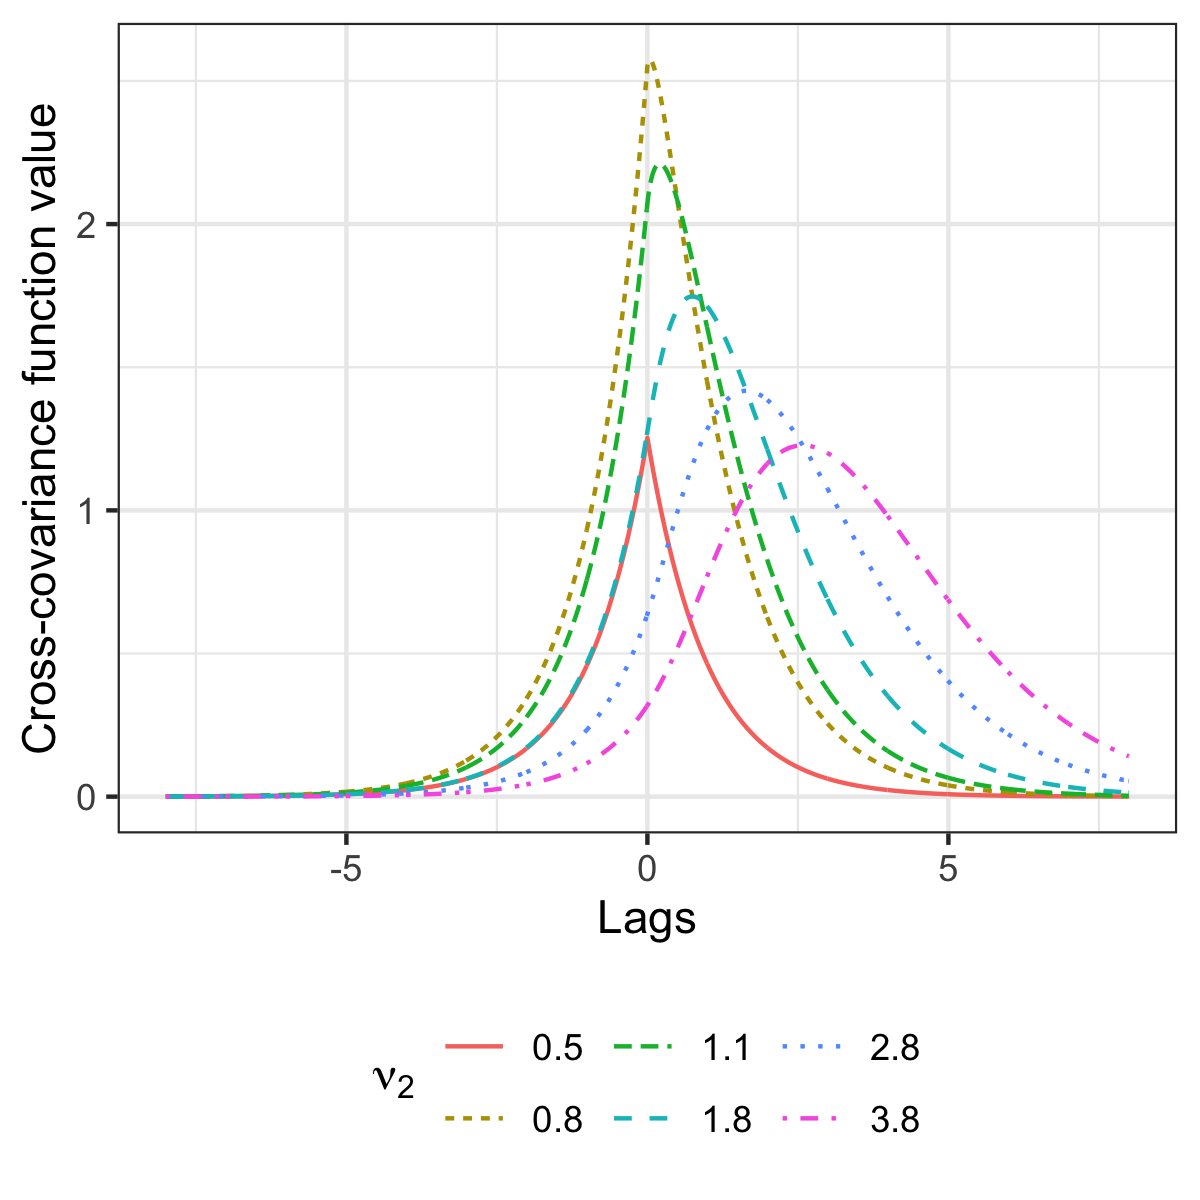
\includegraphics[scale = .16]{../example_fun_whittaker.png}
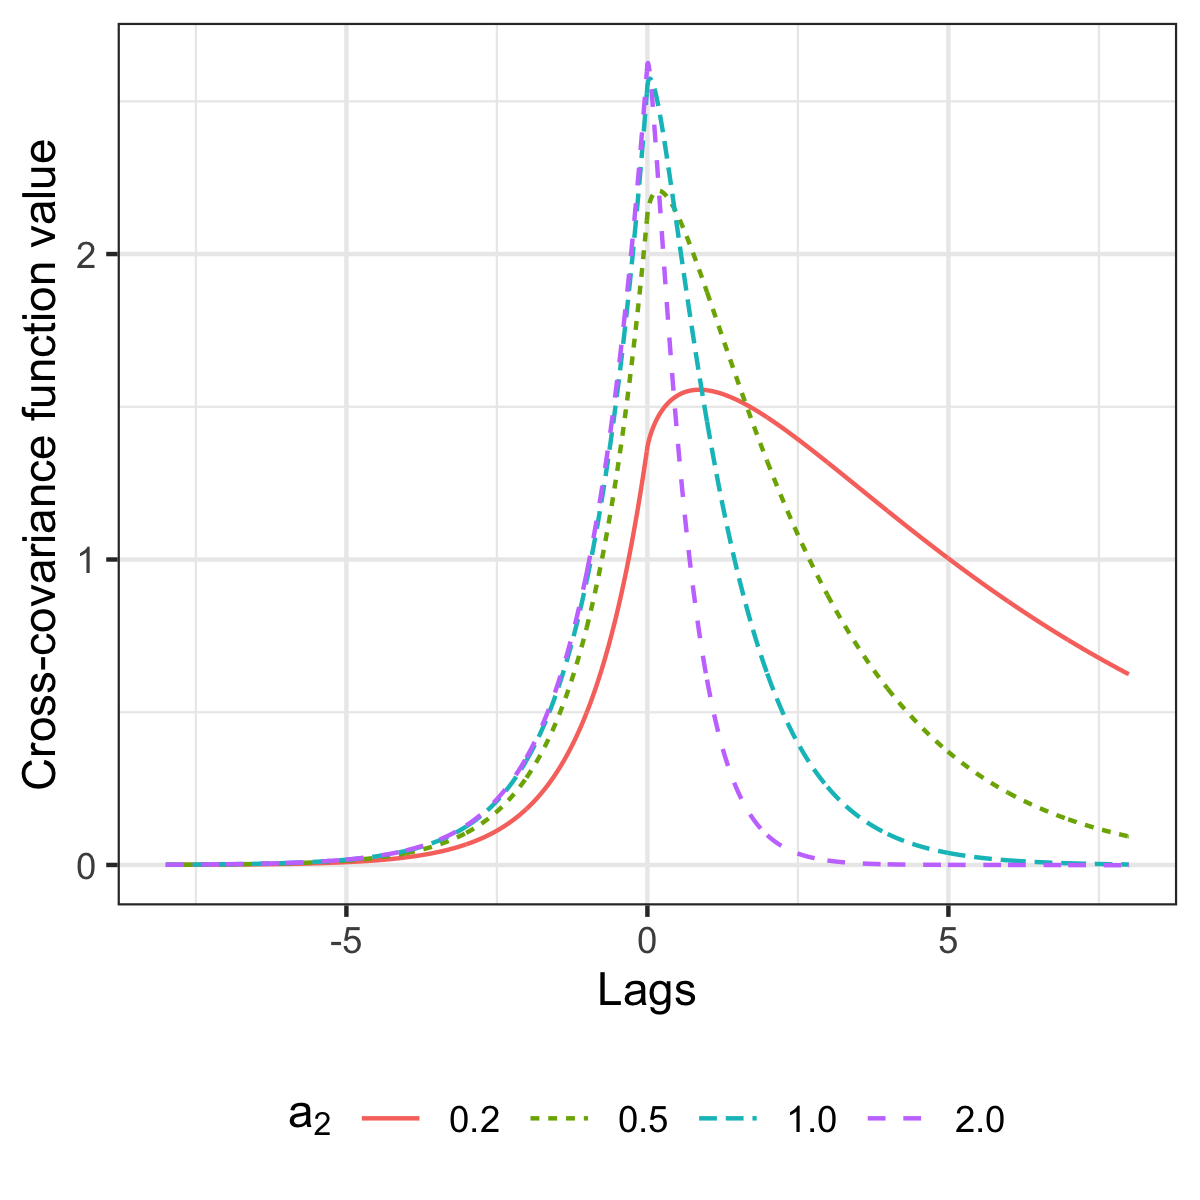
\includegraphics[scale = .16]{../example_fun_whittaker_scale.png}
\caption{Cross-covariance with real entries (Left) Holding $a_1 = a_2 = 1$ and $\nu_1= 0.5$, we plot the cross-covariance function when varying $\nu_2$. (Right) Holding $a_1 = 1$, $\nu_1= 0.5$, $\nu_2 = 0.8$, we plot the cross-covariance function when varying $a_2$.}\label{fig:type_pos}
\end{figure}

By setting $\textrm{Im}(\Sigma_{12}) = 0$, we provide a model that links two Mat\'ern processes with a natural description of the cross-dependence. 
This new family of cross-covariance functions breaks the symmetry and diagonal-dominance assumptions of the multivariate Mat\'ern of \cite{gneiting_matern_2010} through imbalances between $\nu_1$ and $\nu_2$ or, alternatively, $a_1$ and $a_2$.
It is only necessary to estimate one additional parameter, $\textrm{Re}(\Sigma_{12})$, compared to estimating the processes independently. 
Validity of the cross-covariance model is immediately available when $\Sigma$ is positive definite. 
These properties make this model more attractive in multiple aspects compared to that of \cite{gneiting_matern_2010} for modeling multivariate processes. 

\subsection{Cross-covariance with imaginary entries}\label{sec:im_ent}

We now turn to cases where $\textrm{Im}(\Sigma_{12})\neq 0$, which opens up an additional class of multivariate cross-covariance functions. 
Unfortunately, a full description of such models is elusive, and we make the assumption throughout that $a_1 = a_2$. 
We focus first on the case where $\nu_1 = \nu_2$, and in the Appendix demonstrate a more general form for when $\nu_1 - \nu_2$ is an integer. 
Expressions when $\nu_1 - \nu_2$ is not an integer and when $a_1 \neq a_2$ require future work in mathematical analysis.

On the other hand, even with these restrictions, we introduce further flexibility in multivariate Mat\'ern models, as we discuss here. 

\begin{theorem}\label{thm:im_ent}
Suppose that $\nu_1 = \nu_2 > 0$, $\textrm{Re}(\Sigma_{12}) = 0$, and $a_1 = a_2 > 0$. Then the cross-covariance function is written in closed form as \begin{align*}
-\textrm{Im}(\Sigma_{12})c_1\textrm{sign}(h)\left(\frac{|h|}{a_1}\right)^{\nu_1} \left(I_{\nu_1}(a_1|h|) - L_{-\nu_1}(a_1|h|)\right) 
\end{align*}where
%Using \cite{noauthor_table_2015} 3.771 2, we have \begin{align*}
%\mathbb{E}\left(Y(t) Y(s)^*\right) &=-\textrm{Im}(D_{12})c_1\textrm{sign}(h)|h|^{\nu_1} \left(I_{\nu_1}(|h|) - L_{-\nu_1}(|h|)\right) 
%\end{align*}where 
$c_1 =  \frac{\sqrt{\pi}}{2^{\nu_1}}\Gamma(-\nu_1 + 1/2)$, 
$I_\nu(t)$ is the modified Bessel function of the first kind, and 
$L_\nu(t)$ is the modified Struve function. This cross-covariance is valid for $\nu_1 > 0$ except when $\nu_1 = n/2$ for $n \in \mathbb{N}$.

\end{theorem}

\begin{proof}
In this case, based on \eqref{impart2} we write \begin{align*}
\mathbb{E}\left(Y_1(t) Y_2(s)^*\right)
&=i\textrm{Im}(\Sigma_{12})\int_0^\infty e^{ihx}(a_1^2 + x^2)^{-\nu_1 - 1/2} dx  -i\textrm{Im}(\Sigma_{12})\int_{-\infty}^0 e^{ihx}(a_1^2 + x^2)^{-\nu_1 - 1/2} dx \\
&=-2\textrm{Im}(\Sigma_{12})\int_0^\infty \sin(hx)(a_1^2 + x^2)^{-\nu_1 - 1/2}dx\\
&=-2\textrm{Im}(\Sigma_{12})\textrm{sign}(h)\int_0^\infty \sin(|h|x)(a_1^2 + x^2)^{-\nu_1 - 1/2}dx\end{align*}using the identity $e^{ix} = \cos(x) + i\sin(x)$ and the even and odd properties of cosine and sine.


The proof is then a direct application of \cite{noauthor_table_2015} 3.771 (1), which also gives the necessary conditions on $\nu_1$.
\end{proof}

As before, we comment to provide more insight about this formula.

\begin{figure}
\centering
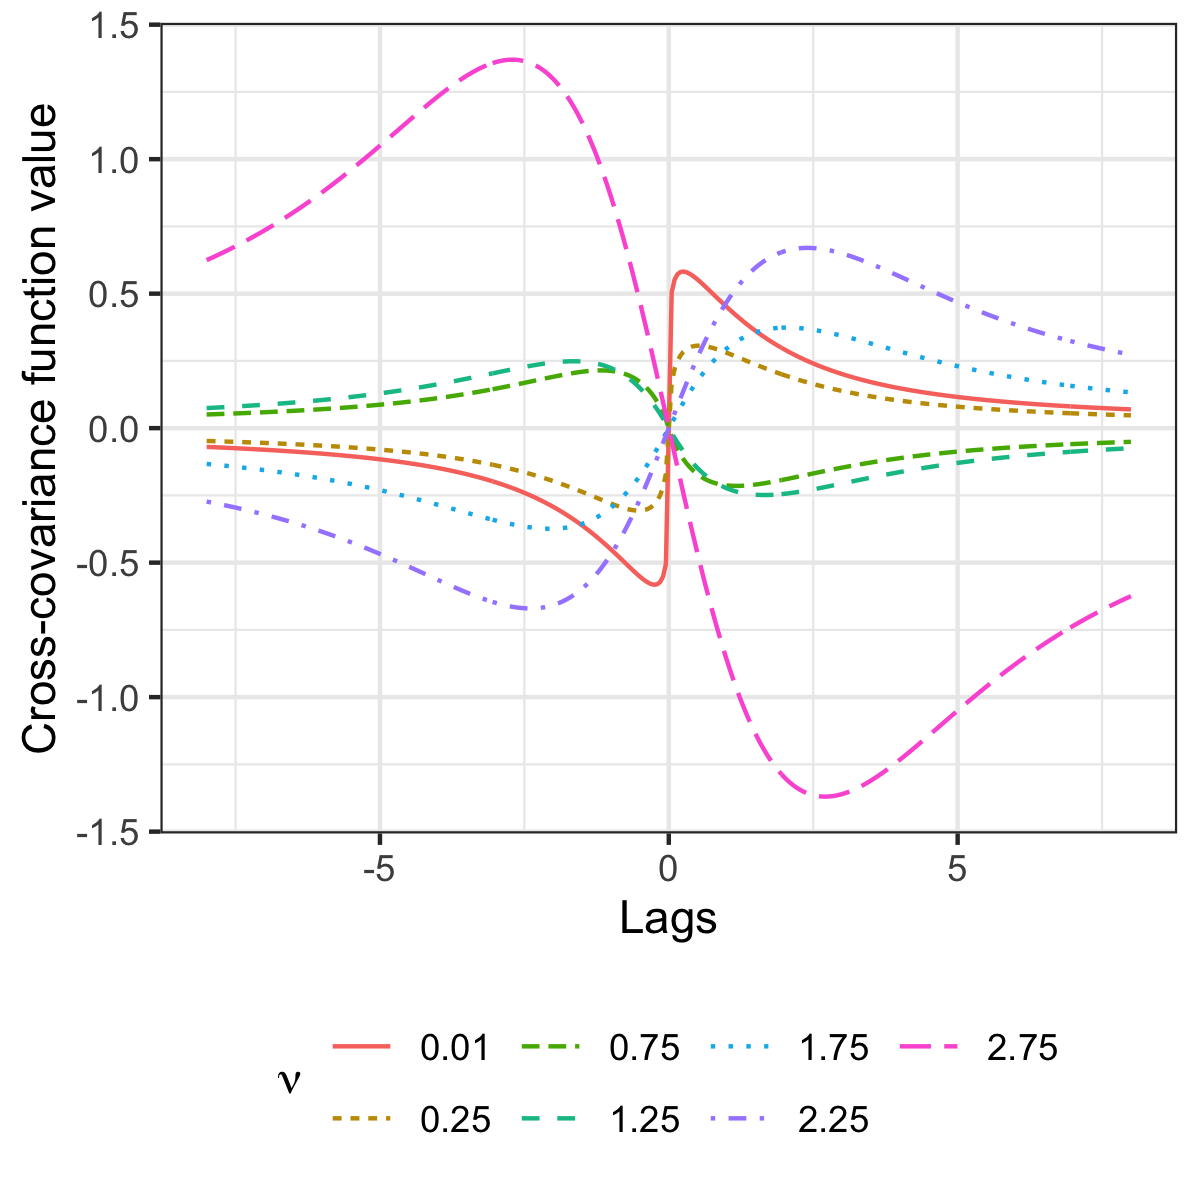
\includegraphics[scale = .15]{../example_fun.png}\label{fig:re_ent}
\caption{The function $\textrm{sign}(h)|h|^{\nu_1} \left(I_{\nu_1}(|h|) - L_{-\nu_1}(|h|)\right)$ for various $\nu_1$. The sign of $I_{\nu_1}(|h|) - L_{-\nu_1}(|h|)$ flips at $\nu_1 = n/2$ for $ n\in \mathbb{N}$.}
\end{figure}


\begin{remark}[Plotted Examples]\normalfont
In Figure \ref{fig:re_ent}, we plot cross-covariance functions. The cross-covariance functions break the uniformity of dependence since they are odd functions. 
\end{remark}

\begin{remark}[Restriction on $\nu_1$]\normalfont
Since $L_{-n - \frac{1}{2}}(h) = I_{n + \frac{1}{2}}(h)$ for $n \in \mathbb{Z}$ \citep[as in 11.4.4 of][]{NIST:DLMF}, the condition that $\nu_1 \neq n/2$ only suggests that there is no contribution to the cross-covariance for $\nu_1 = \frac{1}{2}, \frac{3}{2}, \dots$ based on the $\textrm{Im}(\Sigma_{12})$ term. 
\end{remark}

\begin{remark}[Implementation]\normalfont
The function $I_\nu$ is implemented as \texttt{besselI} in the \texttt{base} package of R, \texttt{iv} in \texttt{scipy} in Python, \texttt{besseli} in Matlab, and \texttt{besselI} in Mathematica. 
The function $L_\nu$ is implemented as \texttt{struveL} in the \texttt{RandomFieldsUtils} package of R, \texttt{modstruve} in \texttt{scipy} in Python, and \texttt{StruveL} in Mathematica. 
\end{remark}

When taking $\textrm{Im}(\Sigma_{12}) \neq 0$, we provide additional Mat\'ern cross-covariance functions when $a_1=a_2 >0$ and $0<\nu_1 = \nu_2 \neq n/2$ for $n \in \mathbb{Z}$. As before, additional scale and smoothness parameters do not need to be estimated. 

\subsection{Review of these two models}

While in Theorem~\ref{thm:re_ent}, we assume $\textrm{Im}(\Sigma_{12}) = 0$ and in Theorem~\ref{thm:im_ent} we assume $\textrm{Re}(\Sigma_{12}) = 0$, it is not necessary to have one be the case. If they are both nonzero, the cross-covariance is the sum of the respective contributions. The resulting cross-covariance will be valid as long as the individual parts are valid and $AA^*$ is positive definite. Such combinations provide a large class of potential shapes in the cross-covariance functions, shown, for example in Figure~\ref{fig:combo_ent}. In Figure~\ref{fig:simulation}, we plot realizations of the multivariate Mat\'ern process. 
\begin{figure}
\centering
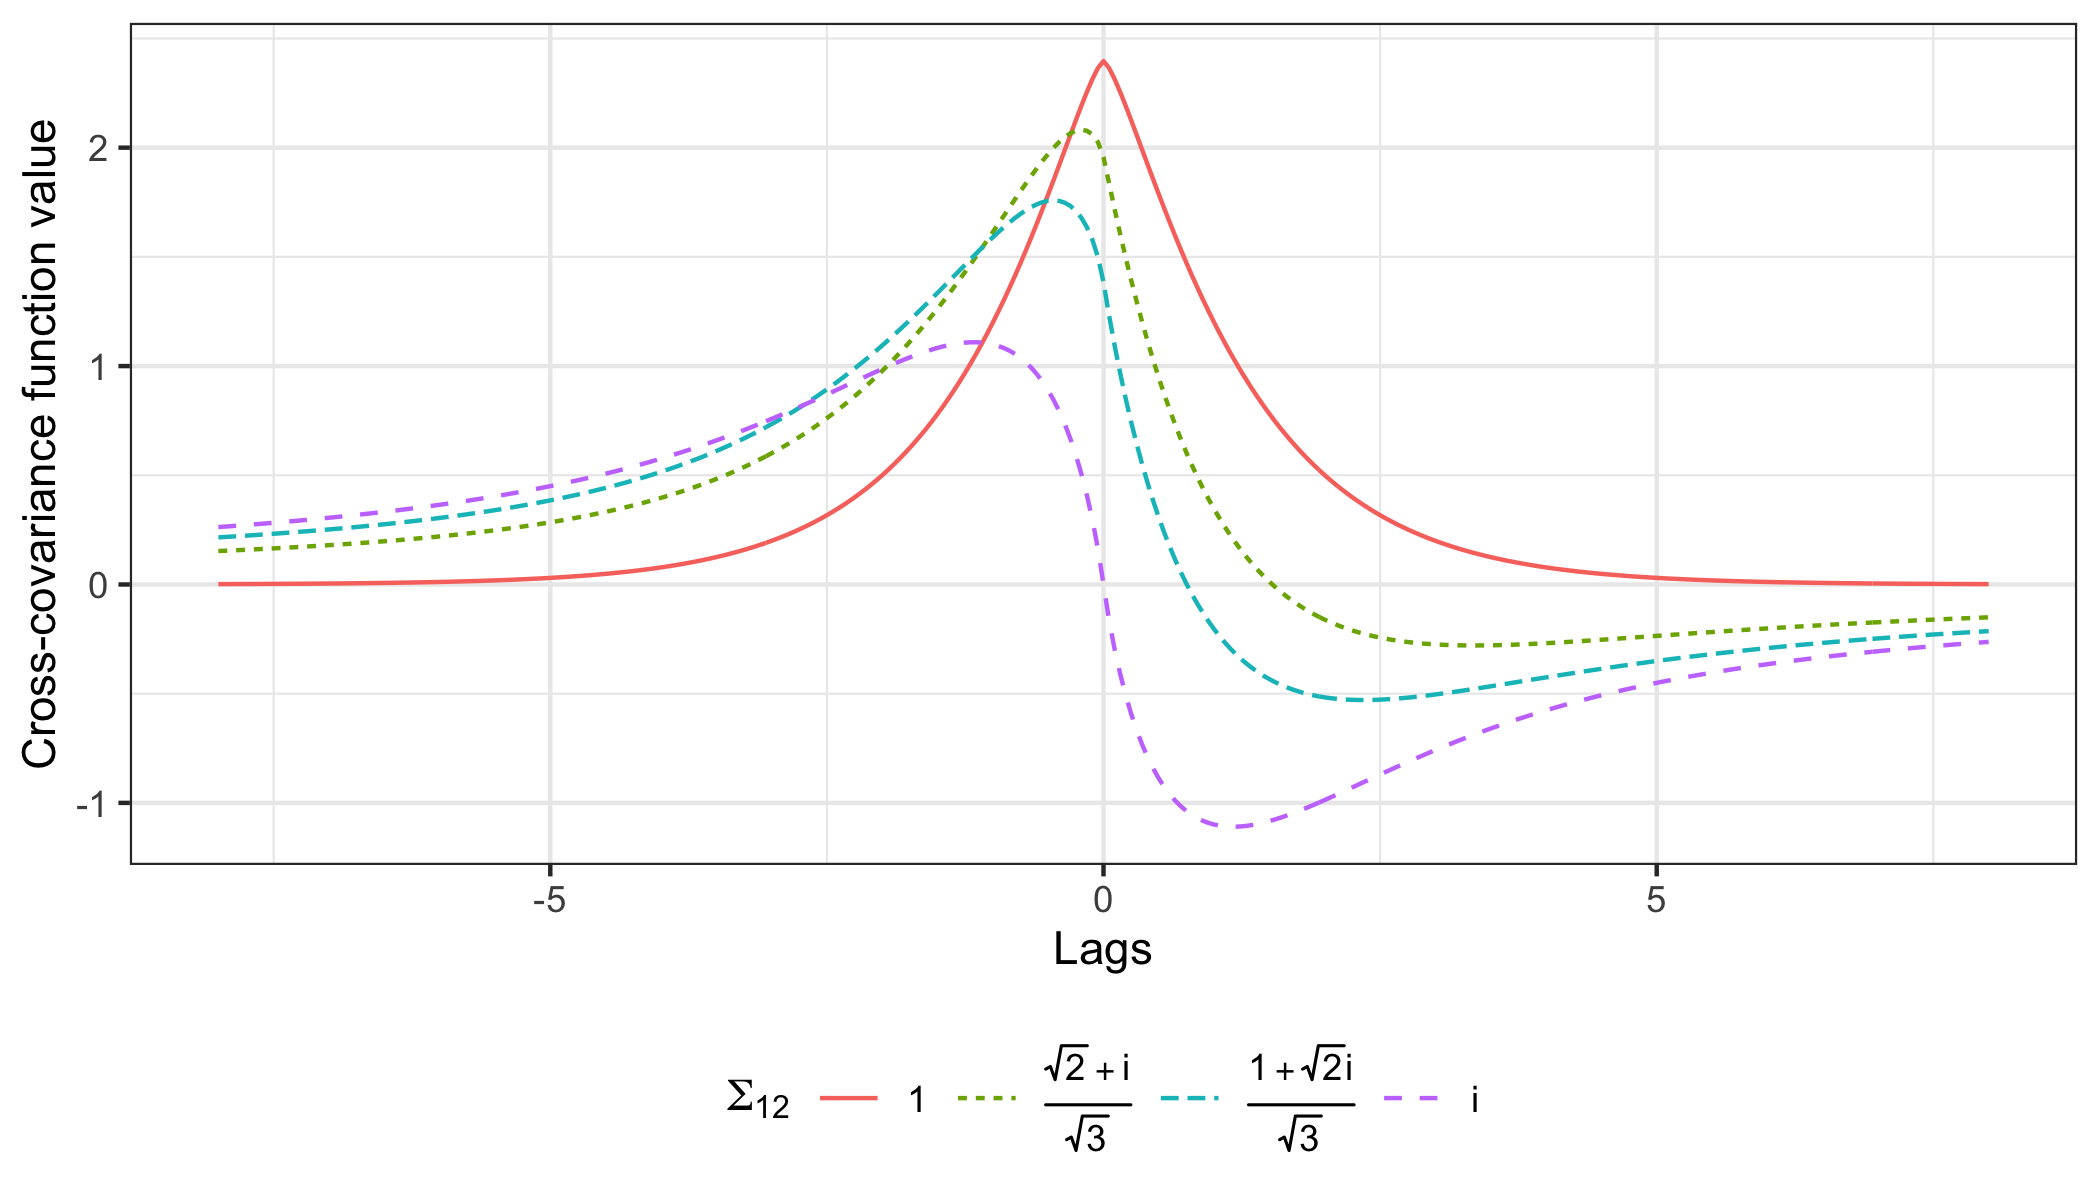
\includegraphics[scale = .15]{../example_combination_function.png}
\caption{Multivariate Mat\'ern cross-covariances for varying values of $\Sigma_{12}$, with $\nu_1 = \nu_2 = 0.75$ and $a_1 = a_2 = 1$. }\label{fig:combo_ent}
\end{figure}
\begin{figure}
\centering
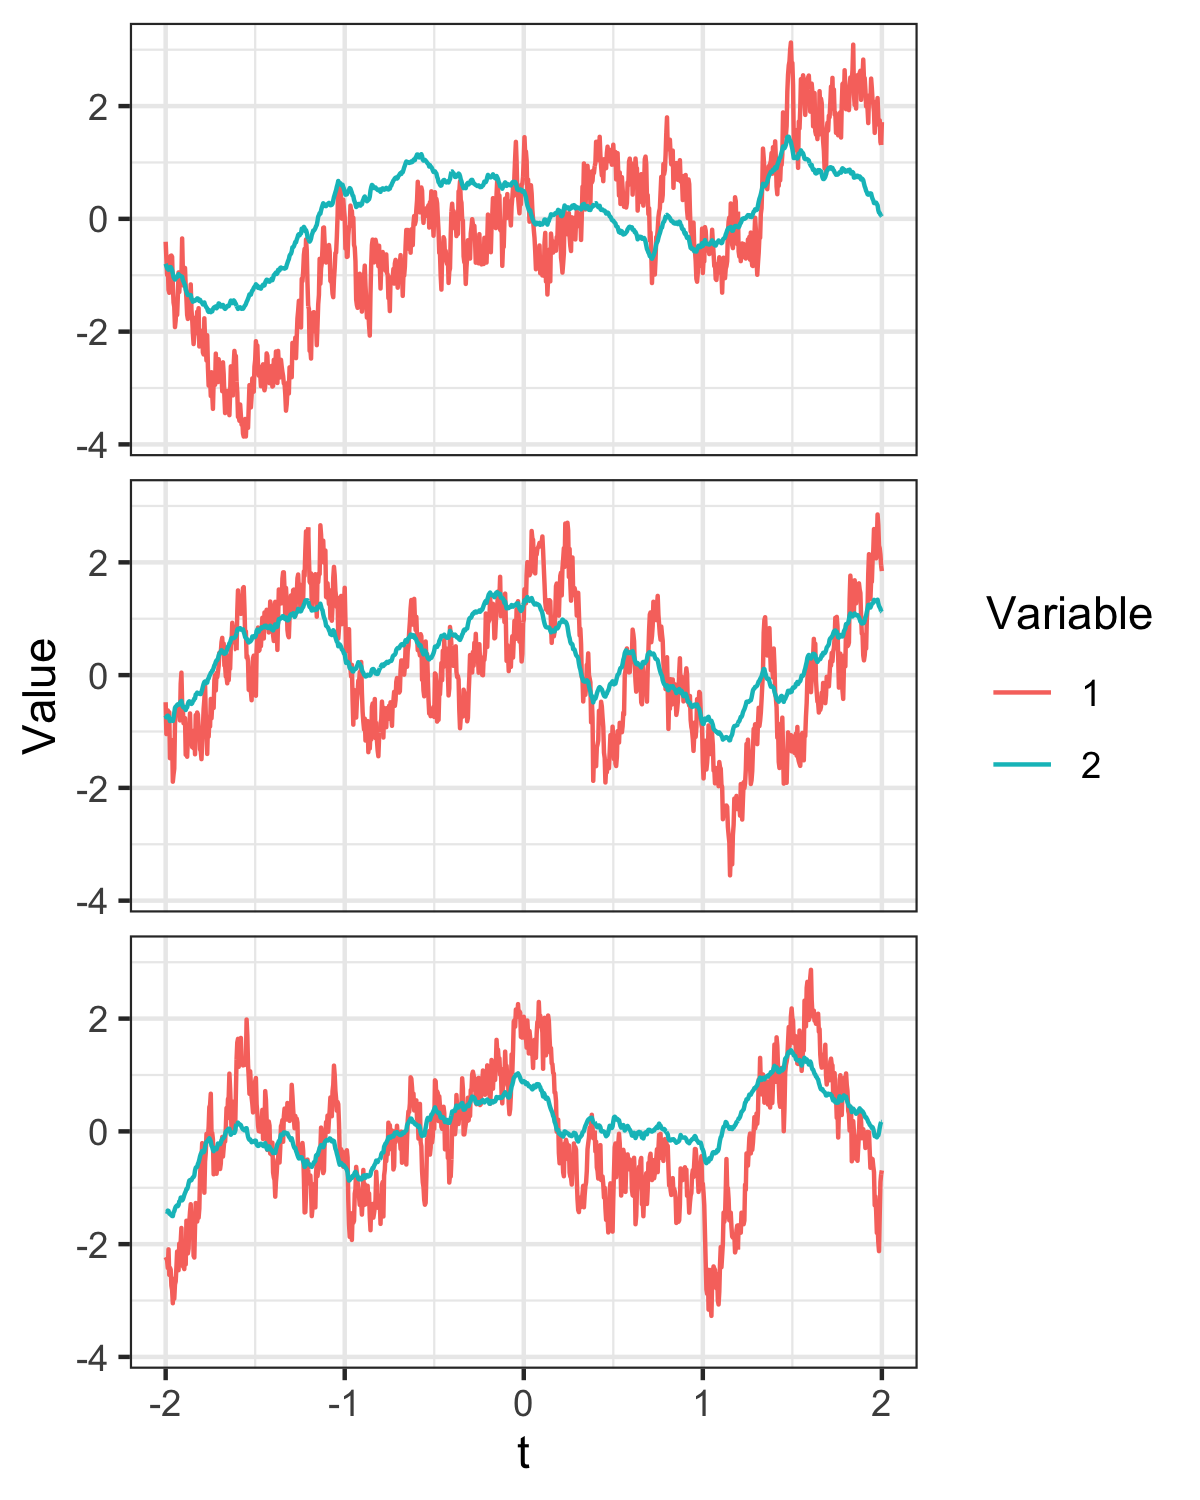
\includegraphics[scale = .15]{../example_simulation.png}
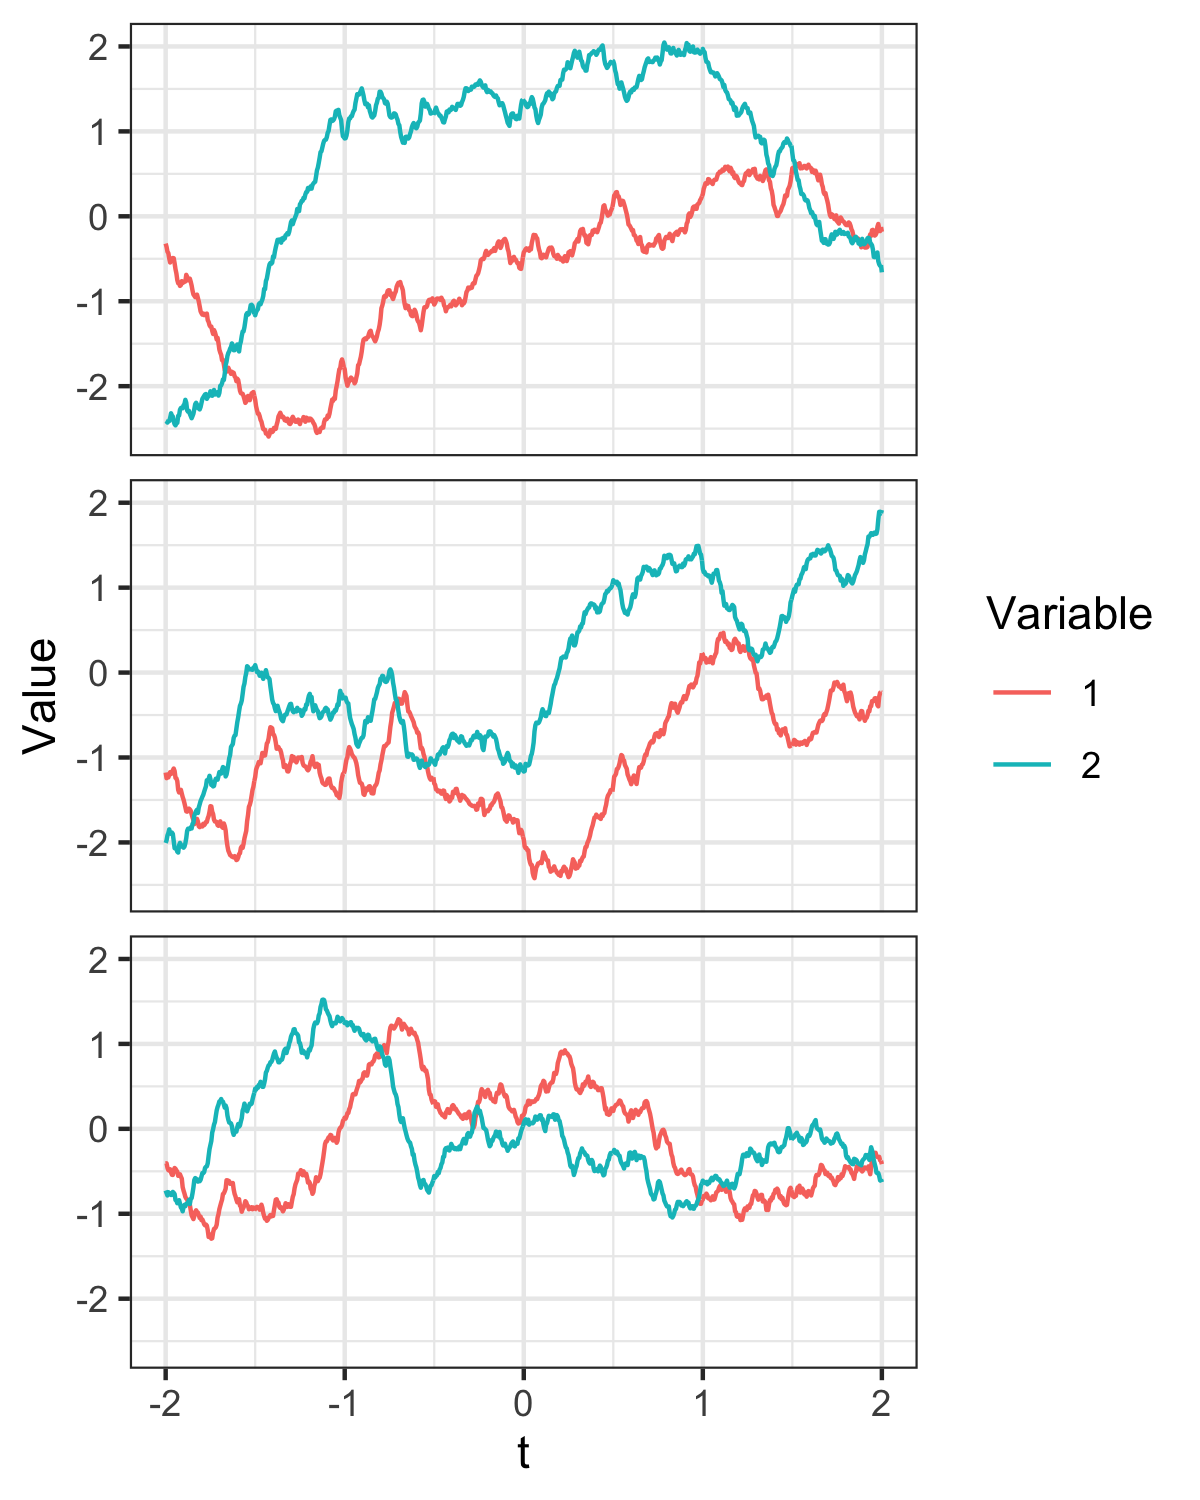
\includegraphics[scale = .15]{../example_simulation_asymm.png}
\caption{Three realizations of multivariate Mat\'ern processes, with $a_1 = a_2 = 1$ and $\Sigma_{11} = \Sigma_{22} = 1$: (Left) With real entries, for $\nu_1 = 0.4$, $\nu_2 = 0.8$, and $\Sigma_{12} = 0.95$. (Right) With imaginary entries, for $\nu_1 = \nu_2 = 0.8$ and $\Sigma_{12} = 0.95i$.}\label{fig:simulation}
\end{figure}

% \begin{remark}[Plotted Examples]\normalfont
% See \url{https://argo.stat.lsa.umich.edu/shiny/ShinyApps/multivariate_matern/} to see various plots of the covariances and cross-covariances.
% \end{remark}


On the other hand, there is still some room open for further models. It is unclear if a closed form of the cross-covariance function exists when $a_1 \neq a_2$ or $\nu_1 - \nu_2$ is not an integer. 


We next consider a discussion of time-reversibility and these cross-covariance models.

\begin{proposition}
In $d=1$, the process is time-reversible iff $\nu_1 = \nu_2$, $a_1 = a_2$, and $\textrm{Im}(\Sigma_{12}) = 0$. 
\end{proposition}

By Proposition 5.1 of \cite{didier_integral_2011}, in our setting time-reversibility is equivalent to $\mathbb{E}(Y_1(s)Y_2(t)) = \mathbb{E}(Y_1(t)Y_2(s))$ for $t, s \in \mathbb{R}$. As we've seen in varying plots, any one the conditions being broken will introduce assymmetry in the model. If $\nu_1 = \nu_2$, $a_1 = a_2$, and $\textrm{Im}(\Sigma_{12}) = 0$, the cross-covariance takes the same shape as the Mat\'ern covariance. Therefore, all new cross-covariances proposed in this paper are time-irreversible. 

\begin{itemize}
\item If $\nu_1 \neq \nu_2$, then the cross-covariance function appears to model some sort of lag. If there are large differences in smoothness of the two processes, our model says the cross-covariance should behave in a certain lagged way, which is maybe unexpected. 

\item If $a_1 \neq a_2$, then the dependence for one variable will be elongated, implying that if the process were reversed, things would then be elongated in the opposite direction.

\item When $\textrm{Im}(\Sigma_{12}) \neq 0$ and $\nu_1=\nu_2$, there is asymmetry in terms of the uniformity of dependence.
\end{itemize}
While the multivariate Mat\'ern of \cite{gneiting_matern_2010} defines symmetric cross-covariance functions and thus reversible processes, these new models demonstrate that irreversible processes can be naturally represented for marginally Mat\'ern processes. 


\section{Some technical comments on this model}\label{sec:technical}

We comment on a few intracacies of this model. First, we outline how such processes have tangent processes of operator functional Brownian motion. Then, we consider the coherence of this new model as definied by \cite{kleiber_coherence_2018}. Finally, we suggest maximum likelihood estimation for its parameters and provide a simulation study estimating them. 

\subsection{Tangent fields of the new multivariate Mat\'ern models}

In the following, we will argue that the tangent process to $Y$ above is an operator fBm.  Letting $c\downarrow 0$, consider a matrix exponent $H$  
   (to be determined) and focus on the increment:
   $$
   c^{-H} (Y(ct) - Y(0)) = c^{-H} \int_{\R}  \frac{(e^{ictx} -1)}{ix} \left( ix (1+ix)^{-\nu -1/2}A 1_{\{x>0\}} + i x (1+ix)^{-\nu - 1/2}\overline{A}1_{\{x<0\}}\right) \tilde B(dx).
   $$
   By changing the variables $u := cx$, and using the facts that 
   $$
   iu (c+iu)^{-\nu-1/2} 1_{\pm u>0} \to  (u)_\pm^{-\nu+1/2} e^{ \pm i (1/2 -\nu) \pi/2 } ,\ \mbox{ as }c\downarrow 0,
   $$
   we obtain \fbox{justify the exchange of limits and integration}
   \begin{align*}
  \{ c^{-H} (Y(ct) - Y(0))\} &\eqd\left\{ c^{-H} \int_{\R} c \frac{(e^{itu} -1)}{iu} \left( iu c^{-1} c^{\nu+1/2} ( c + iu)^{-\nu-1/2} {\Big(} A 1_{\{ u>0\}}+ \overline{A} 1_{\{ u<0\}}{\Big)}\right) c^{-1/2}   \tilde B(d u) \right\}\\
   &\stackrel{fdd}{\to} \left \{ \int_{\R} \frac{(e^{itu} -1)}{iu} \left( (u)_+^{-D}A_\nu 1_{\{ u>0\}}+ (u)_-^{-D} \overline A_\nu 1_{\{ u<0\}}\right) \tilde B(d u)\right \},
   \end{align*}
   where we used the fact that $\{B(du/c)\} \eqd\{c^{-1/2} B(du)\}$ and $\stackrel{fdd}{\to}$ means convergence in fdd,
   $$
   D \equiv H- 1/2 := \nu - 1/2\quad \mbox{ and }\quad A_\nu := e^{i (1/2 -\nu) \pi/2 }A.
   $$
   (Note: observe that $(ab)^C = a^C b^C = b^C a^C$ for all $a,b\in\C$ (appropriately defined) while $c^A c^B$ does not always equal $c^B c^A$
   -- unless $A$ and $B$ commute.)  This shows that if we choose 
   $H:=\nu$,
   we obtain that the tangent process to $Y$ is the operator fBm with self-similarity exponent $H\equiv \nu$.
   
   Now, the characterization of \cite{didier_integral_2011} in \eqref{e:diddier-pipiras} shows that the model in \eqref{e:o-Matern} can achieve all possible tangent processes and in this sense it is a complete extension to the Mat\'ern model, where the exponent $\nu$ is replaced by an operator ($k\times k$ matrix) whose eigenvalues have real parts in $(0,1)$.


\subsection{Coherence function}
One way to evaluate the statistical properties of multivariate covariance functions is coherence, as explored in \cite{kleiber_coherence_2018}. 
The measure of coherence evaluates the strength of the linear relationship between two spatial processes at a particular frequency. 
Based on the definition of coherence in \cite{kleiber_coherence_2018} and letting $f_{ij}(x)$ be the $i,j$ entry of the matrix of spectral densities, we write the coherence of the introduced model as \begin{align*}
\gamma(x) &= \frac{f_{12}(x)}{\sqrt{f_{11}(x) f_{22}(x)}} \\ %\frac{(a_1 + ix)^{-\nu_1 - 1/2}(a_2 - ix)^{-\nu_2 - 1/2}(\Sigma_{12}1_{x > 0} + \overline{\Sigma}_{12}1_{x < 0})}{\sqrt{\Sigma_{11}(a_1^2 + x^2)^{-\nu_1 - 1/2}\Sigma_{22}(a_2^2 +x^2)^{-\nu_2 - 1/2}}}\\
&=\frac{(a_1 + ix)^{-\nu_1 - 1/2}(a_2 - ix)^{-\nu_2 - 1/2}(\Sigma_{12}1_{x > 0} + \overline{\Sigma}_{12}1_{x < 0})}{\sqrt{\Sigma_{11}(a_1+ ix)^{-\nu_1 - 1/2}(a_1 - ix)^{-\nu_1 - 1/2}\Sigma_{22}(a_2 +ix)^{-\nu_2 - 1/2}(a_2 -ix)^{-\nu_2 - 1/2}}}\\
&=\frac{\Sigma_{12}1_{x > 0} + \overline{\Sigma}_{12}1_{x < 0}}{\sqrt{\Sigma_{11}\Sigma_{22}}}\frac{\sqrt{(a_1 + ix)^{-\nu_1 - 1/2}(a_2 -ix)^{-\nu_2 - 1/2}}}{\sqrt{(a_1 - ix)^{-\nu_1 - 1/2}(a_2 +ix)^{-\nu_2 - 1/2}}}.
\end{align*}As this is potentially a complex number, \cite{kleiber_coherence_2018} recommends evaluating the squared absolute coherence function: \begin{align*}
|\gamma(x)|^2&= \frac{|\Sigma_{12}|^2}{\Sigma_{11}\Sigma_{22}},
\end{align*}a constant, simple, and interpretable function of $x$. While \cite{kleiber_coherence_2018} suggests that a constant coherence function reflects relative inflexibility, this is perhaps expected when there are few parameters to influence the behavior of the cross-covariance relationship. We also find that, even with a constant coherence function, such processes can have relatively flexible covariance functions. 

\subsection{Maximum Likelihood Estimation}\label{sec:ml_est}

We propose a maximum likeilhood approach to the estimation of the parameters in this model. In particular, we will assume that $Y(t)$ is a vector-valued zero-mean Gaussian Process and covariance parameterized by the new multivariate Mat\'ern model. As before, we focus on the $K=2$ and $d=1$ setting. 

Suppose that we observe $Y(t_i) = \begin{pmatrix}Y_1(t_i) \\ Y_2(t_i)\end{pmatrix}$ where $t_i \in [0,1]$ for $i=1, \dots, n$. Let $C_M(\theta_1) \in \mathbb{R}^{n\times n}$ the Mat\'ern covariance matrix for points $\{t_i\}_{i=1}^n$ with parameters $\theta_1 = (a_1, \nu_1, \Sigma_{11})$, and define parameters $\theta_2 = (a_2, \nu_2, \Sigma_{22})$ similarly. Finally, let $C_{12}(\theta_1, \theta_2, \theta_{12}) \in \mathbb{R}^{n\times n}$ denote the new Mat\'ern cross-covariance presented in this paper at points $\{t_i\}_{i=1}^n$, with parameters $\theta_1$, $\theta_2$, and $\theta_{12} = (\textrm{Re}(\Sigma_{12}), \textrm{Im}(\Sigma_{12}))$. Then, the normality assumption gives \begin{align*}
Y:=\begin{pmatrix}
\{Y_1(t_i)\}_{i=1}^n \\
\{Y_2(t_i)\}_{i=1}^n
\end{pmatrix}\sim \mathcal{N}\left(0, C(\theta) := \begin{pmatrix}
C_M(\theta_1) & C_{12}(\theta_1, \theta_2, \theta_{12}) \\
C_{12}(\theta_1, \theta_2, \theta_{12})^\top & C_M(\theta_2)
\end{pmatrix}\right)
\end{align*}so that the log-likelihood function of the data is \begin{align*}
\ell(\theta) &= -\frac{Kn}{2} \log(2\pi) - \frac{1}{2}Y^\top C(\theta)^{-1} Y - \frac{1}{2}\log(|C(\theta)|)
\end{align*}where $|C(\theta)|$ is the determinant of $C(\theta)$. The determinant and inverse of $C(\theta)$ can be computed using $n\times n$ matrix inversion using the Schur complement an properties of block matrices. For example, \begin{align*}
|C(\theta)| &= |C_M(\theta_1)| \cdot |C_M(\theta_2) - C_{12}(\theta_1, \theta_2, \theta_{12})^\top C_M(\theta_1)^{-1}C_{12}(\theta_1, \theta_2, \theta_{12})|.
\end{align*}

% \begin{itemize}
% \item Find gradients and Hessian with respect to $\Sigma_{12}$ and other parameters
% \item Does information about one process tell you anthing about the parameters of the other?
% \end{itemize}

%\section{Testing if the process is reversible}

\subsection{Simulation}\label{sec:simulation}

We consider a simulation study to assess parameter estimation and the model. In this study, we aim to investigate the potential identifiability and estimation error of the parameters. Since in the univariate Mat\'ern model, $\Sigma_{11}$ and $a_1$ are not simultaneously identifiable \citep{zhang_inconsistent_2004}, we take $a_1 = a_2 = 1$ as known. 
For simplicity, we assume $t_i = \frac{i}{n}$ are observed on a regular grid, and we consider $ n= 100, 150, 200, 250, 300, 350$, and $400$. For each sample size, we consider $200$ replicates.  
In addition, we evaluate three different estimation strategies for the parameters: {\bf a)} estimation of $\theta$ simultaneously {\bf b)} estimation of $\theta_k$ using only data from the $k$-th process, then estimating $\Sigma_{12}$ with $\theta_1$ and $\theta_2$ fixed {\bf c)} using the estimates of $\theta_k$ as in b) as the initial values for the estimation approach of a). The L-BGGS-B optimization methodology was used for maximum likelihood estimation for the parameters, and a log-transform was used for all parameters except those governing $\Sigma_{12}$.

We consider three simulation setups, each with $\Sigma_{11} = \Sigma_{22} = 1$.
For the first simulation, we consider $\Sigma_{12} = 0.8$, $\nu_1 = 0.4$, and $\nu_2 = 0.8$. This reflects moderately strong dependence between the processes that have varying smoothness. In this setting, we assume that $\textrm{Im}(\Sigma_{12}) = 0$. In the second simulation, we consider $\Sigma_{12} = 0.8i$, $\nu_1 = 0.8$, and $\nu_2 = 0.8$ to evaluate performance when $\Sigma_{12}$ is imaginary. In the final simulation study, we consider $\Sigma_{12} = 0.3 + 0.3i$ with the parameters $\nu_1 = \nu_2 = 0.8$. We consider the root-mean-squared-error, the bias $\overline{\theta} - \theta$, and the standard deviation $\sqrt{\frac{1}{200}\sum_{i=1}^{200} (\hat{\theta}_i - \overline{\theta})^2}$, where $\overline{\theta} = \frac{1}{200}\sum_{i=1}^{200} \hat{\theta}_i$.

Results for these two simulations are plotted in Figure \ref{fig:simu}, and for the final simulation we show results in Table~\ref{tab:simu_both}. Overall, increasing sample size reduces the error in each of the parameter estimates. The variance primarily contributes to the error in the estimates, while there is very little bias in estimating each of the parameters.

\begin{figure}[h]
\centering
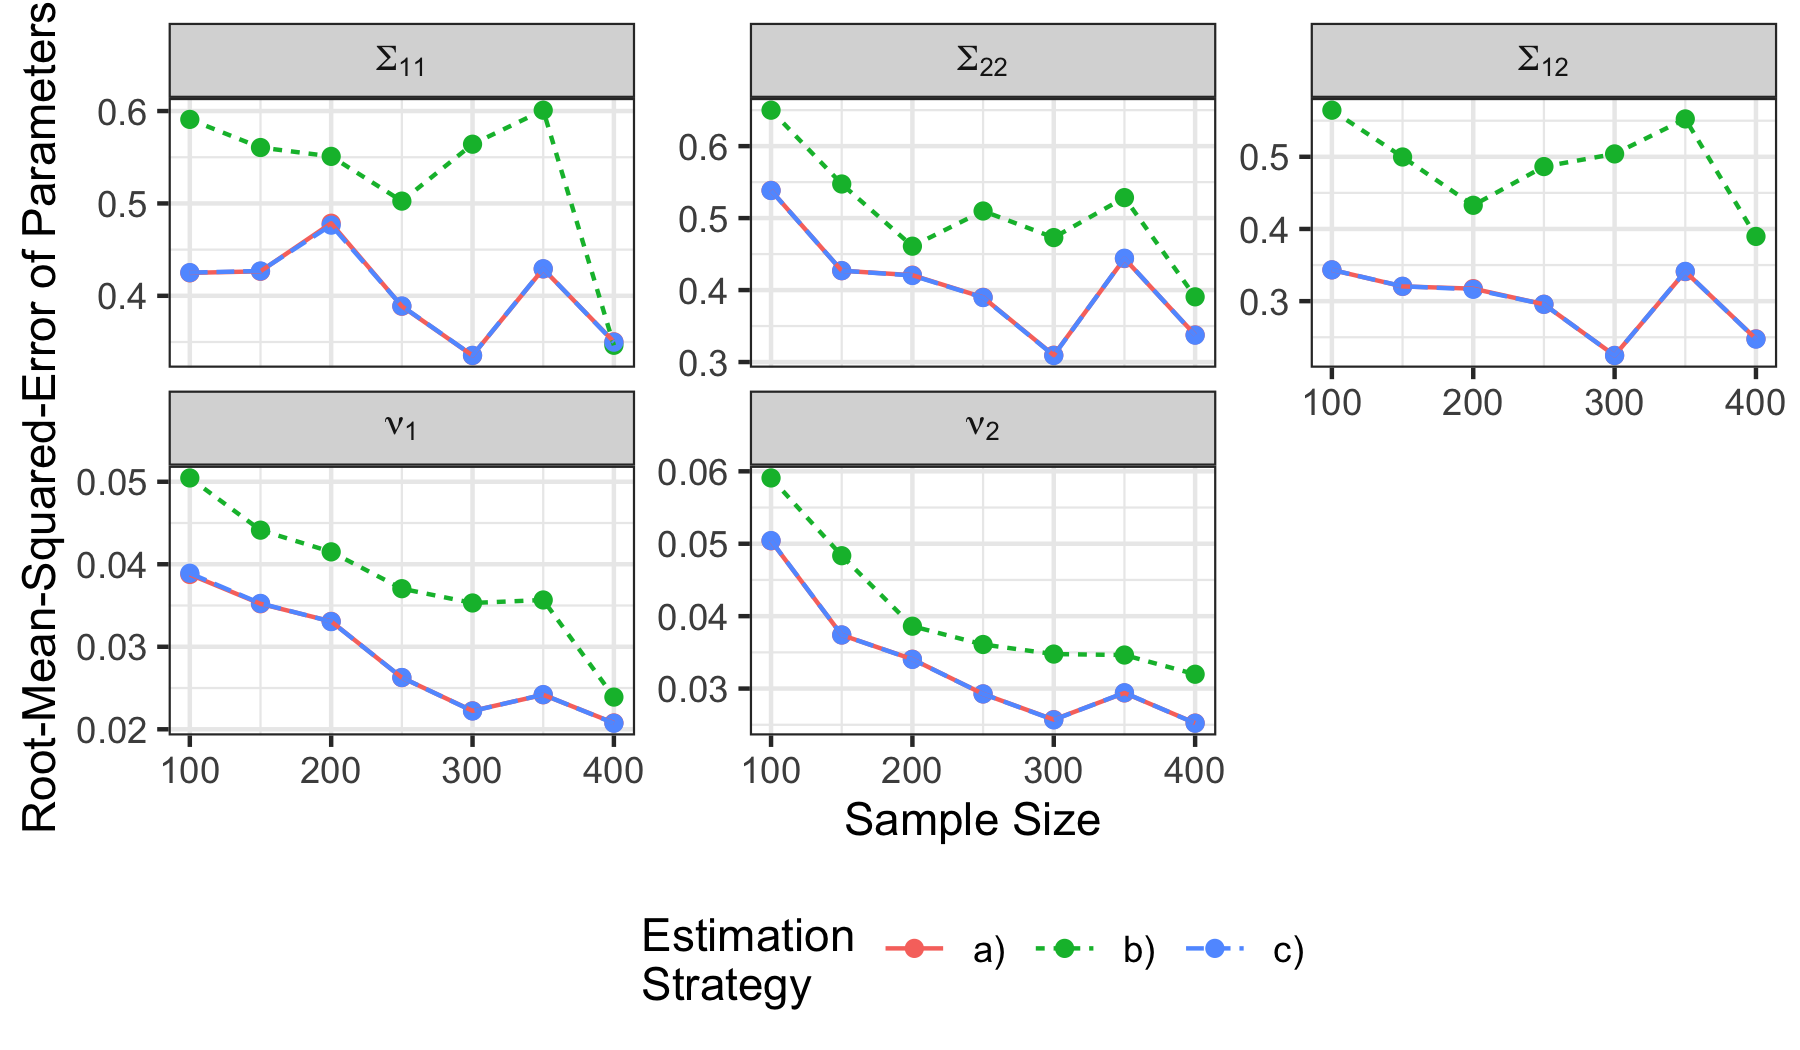
\includegraphics[scale=.11]{../simulation_plot_real.png}
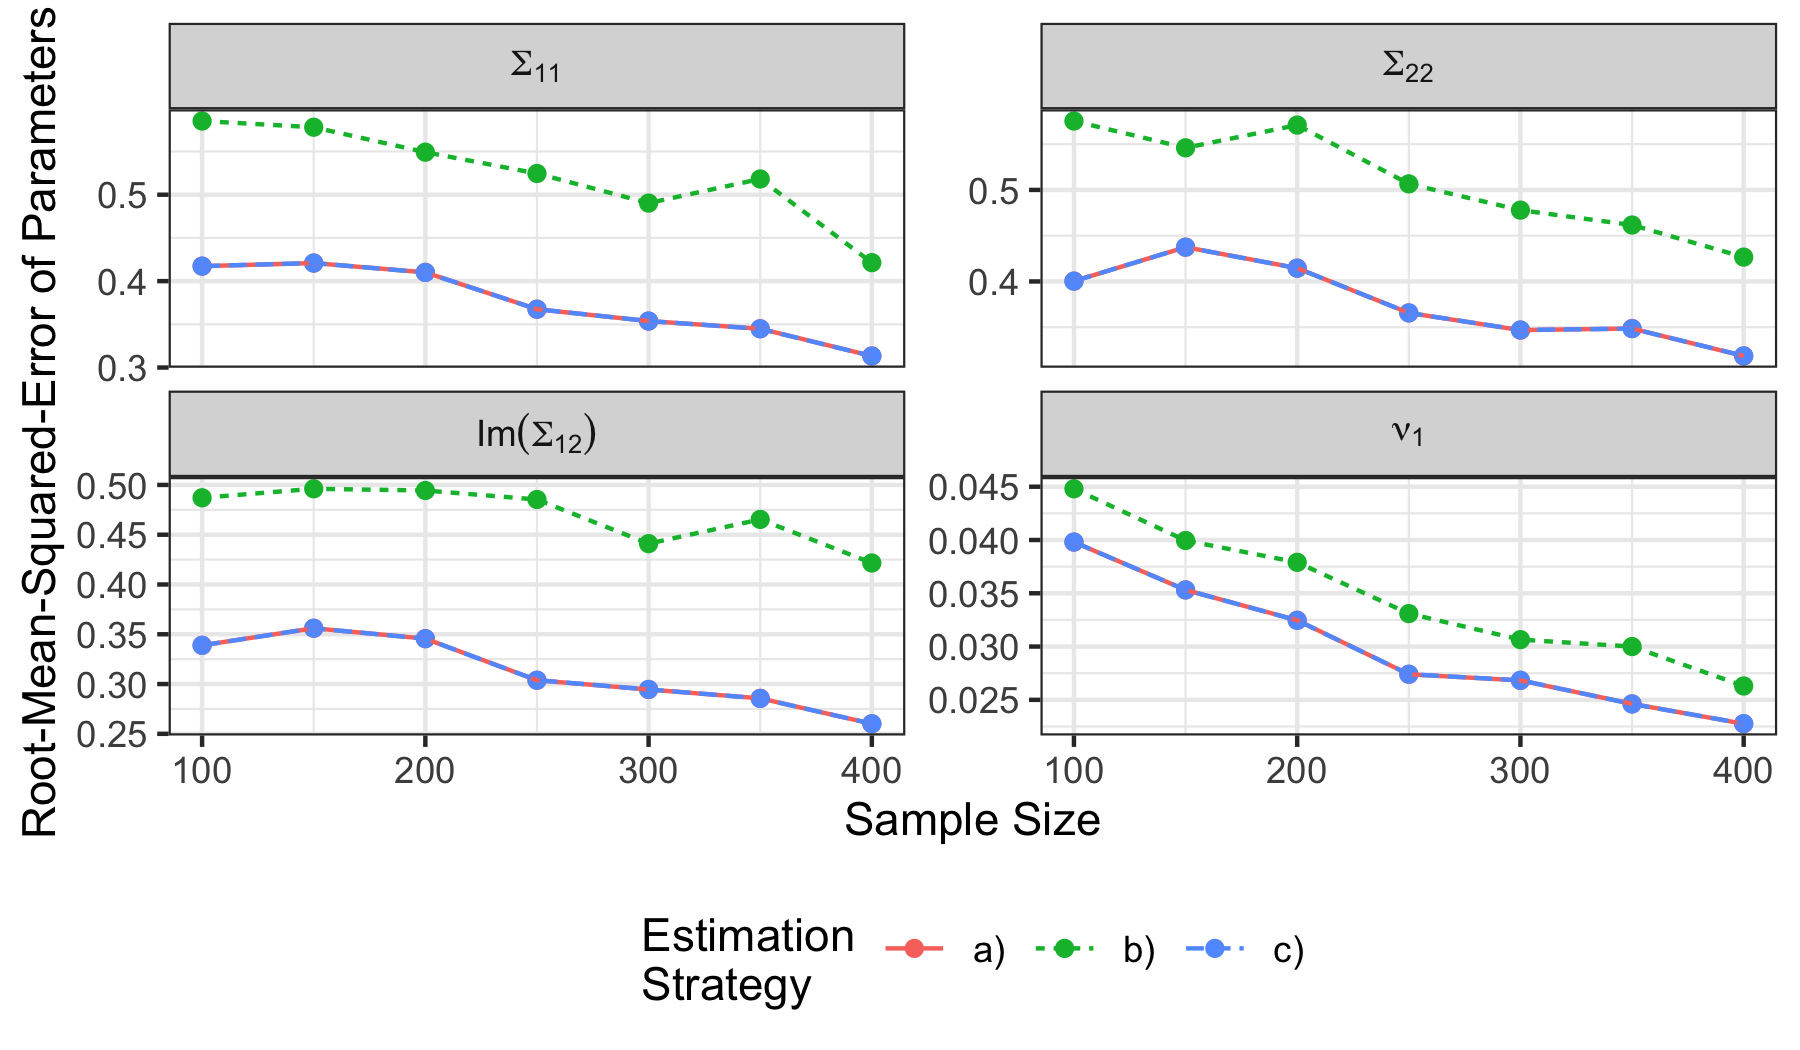
\includegraphics[scale=.11]{../simulation_plot_imaginary.png}
\caption{Root-mean-squared-error in estimating the parameters for varying sample sizes, across 200 simulations. (Left) With real entries (Right) With imaginary entries.}\label{fig:simu}
\end{figure}


\begin{table}[h]

\begin{tabular}{|c|c|c|c|c|c|c|c|c|}\hline
Parameter & Error & $n= 100$ & $n= 150$ & $n= 200$ & $n= 250$ & $n= 300$ & $n= 350$ &$n= 400$  \\
\hline\hline
Re$(\Sigma_{12})$ &Bias & 0.016& 0.014 &0.014  &0.015  &-0.002  & 0.012 & 0.002 \\  \hline
Re$(\Sigma_{12})$& SD & 0.160 & 0.151 & 0.138 & 0.123 & { }0.105 & 0.110 & 0.101 \\  \hline\hline
Im$(\Sigma_{12})$&Bias & 0.003 & 0.030 & 0.023 & 0.021 & { }0.003 & 0.018 & 0.015 \\  \hline
Im$(\Sigma_{12})$&SD & 0.168 & 0.173 &  0.157 & 0.133 & { }0.131 & 0.128 & 0.116 \\  \hline
\end{tabular}
\caption{Estimation of covariance parameters where $\Sigma_{12} = 0.3 + 0.3i$. There is little bias and the variance of estimates decreases as the sample size increases. The variance in estimating $\textrm{Im}(\Sigma_{12})$ is slightly larger than the variance in estimating $\textrm{Re}(\Sigma_{12})$.}\label{tab:simu_both}
\end{table}

% Compare: \begin{itemize}
% \item Sample size, estimation strategy, parameter
% \item log-likelihood
% \item coverage
% \item length
% \item error
% \end{itemize}


% Further points to consider:
% \begin{itemize}
% \item Prediction/cokriging
% \item Compare with other multivariate Mat\'ern models
% \end{itemize}

%``We consider two predictive scores, the logarithmic score (LogS) and the continuous ranked probability score (CRPS), proposed by Gneiting and Raftery (2007) and Gneiting, Balab- daoui, and Raftery (2007) and described by Zhang and Wang (2010) in the context of large datasets.''

\section{Approaching a functional model}\label{sec:functional}

In many applications, spatial statistics for functional data as taken renewed interest; for example, see \cite{martinez-hernadez_recent_2020} and references therein. Here, we attempt to expand the multivariate model we developed here into a functional one. Consider a $\mathbb{R}^K$ multivariate Mat\'ern model with parameters defined as follows. We set $a_{k} = a_f(k/K)$ for some function $a_f : [0,1] \to \mathbb{R}^+$ and $\nu_k = \nu_f(k/K)$ for some function $\nu_f: [0,1] \to \mathbb{R}^+$. Next, construct a postive-definite functional covariance operator $C_f(\cdot,\cdot): [0,1]^2 \to \mathbb{R}$; more information on such operators can be found in \cite{hsing_theoretical_2015}. Construct the matrix $\Sigma = \{C_f(k_1/K, k_2/K)\}_{k_1, k_2 = 1}^K \in \mathbb{R}^{K\times K}$.
These parameters chosen represent a valid multivariate Mat\'ern model, and denote a realization of such a process by $Y^{(K)}(t) \in \mathbb{R}^K$. 
Furthermore, denote the 2-dimensional function $\mathcal{K}^{(K)}(p_1,t_1;p_2,t_2) = \mathbb{C}\textrm{ov}( Y^{(K)}_{\lfloor Kp_1\rfloor}(t_1), Y^{(K)}_{\lfloor Kp_2\rfloor}(t_2))$. As $K$ increases, the discretization gets smaller with respect to $p$. 

We refer to a \textit{multivariate-generated functional Mat\'ern process} with parameters $C_f$, $a_f$, and $\nu_f$ as the class of processes from $[0,1] \times \mathbb{R} \to \mathbb{R}$ with covariance function \begin{align*}
\mathcal{K}(p_1,t_1;p_2,t_2)=\lim_{K\to \infty} \mathcal{K}^{(K)}(p_1,t_1;p_2,t_2).
\end{align*}
Each individual $\mathcal{K}^{(K)}(p_1,t_1;p_2,t_2)$ is not a valid covariance function, since constructing a covariance matix with gaps of $p$ smaller than $1/K$ yields a non-invertible matrix. However, as $K \to \infty$, we attain convergence to a positive definite function and thus a valid covariance. Also, since $C_f$ must be real-valued, $AA^*$ does not have any imaginary entries. Finally, one can estimate a $K$-dimensional representation of the parameters $C_f$, $a_f$, and $\nu_f$ by estimating the multivariate Mat\'ern parameters.

%As evaluation of this covariance for a set of high-resolution data in $p$ would need to consider large $K$ and would suffer computationally through the factorization of dense matrices. However, some form of finite-dimension representations are necessary what practically applying functional data, so this is not surprising. Furthermore, one can estimate a $K$-dimensional representation of the parameters $C_f$, $a_f$, and $\nu_f$ by estimating the multivariate Mat\'ern parameters. Also, note that since $C_f$ must be real-valued, $AA^*$ does not have any imaginary entries. 

In the functional data literature, it is most common to assume a functional principal component decomposition (FPCA) $C_f(p_1, p_2) = \sum_{k=1}^K \lambda_k \phi_k(p_1) \phi_k(p_2)$, then model the dependence in $t$ for each $k$ separately. For example, see \cite{martinez-hernadez_recent_2020} and references therein. One advantage of this approach is dimension reduction, as only a moderate $K$ may be necessary to capture the variability of interest. In particular, if $m$ data points in $p$ are observed at each of $n$ times, the FPCA approach effectively requires $O(Kn^3)$ floating point operations to compute the Cholesky factor of the covariance matrix of the scores, yet for this new model $O((mn)^3)$ are needed since dimension reduction is unavailable. On the other hand, the FPCs $\phi_k$ are generally estimated to be smooth functions. Thus, it is more challenging to model quick changes in the covariance structure, as the principal component scores represent a weighted average across the domain $p \in [0,1]$. With this new functional Mat\'ern model, non-smooth or discontinuous functions for $\nu_f$ and $a_f$ would provide more flexibility compared to functional-principal-component-based models. 

\section{Characterization of spatial cross-covariances}\label{sec:spatial}

Thus far, we have considered only the time series setting, that is, when $d=1$. The reaches of such a model are limited, and in this section we characterize spatial processes as well. When $d=2, 3, \dots$, such processes are more complicated, and closed-form solutions to the cross-covariances are thus-far elusive to the authors. On the other hand, we demonstrate that integrals can be approximated to represent these processes, and simulation of these processes is possible. In particular, as $d$ increases, there is increased flexiblity in the model in terms of the domain. We demonstrate two cases where the cross-covariance for $d > 1$ is analygous to the $d=1$ case. % In the following, we demonstrate our work in developing such processes. 

We repeatedly refer to \cite{didier_domain_2018} who develop an harmonic integral representations for operator fractional brownian motion for general $d$, namely in (3.24): \begin{align*}
\{X(t)\}_{t\in \mathbb{R}^d}&\overset{d}{=} \int_0^\infty \int_{S_0} (e^{i\langle t, r^{E^*}\theta\rangle} - 1)r^{-H - I/2}\tilde{B}_{H, \Delta}(dr, d\theta)
\end{align*}where \begin{align*}
\mathbb{E}\tilde{B}_{H, \Delta}(dr, d\theta)\tilde{B}_{H, \Delta}(dr, d\theta)^* = dr \Delta(d\theta)
\end{align*}and $\Delta$ is a Hermetian $d \times d$ matrix-valued measure on $S_0$ such that $\Delta(d\theta) = \overline{\Delta}(-d\theta)$. Here, $S_0$ is the unit ball in $\mathbb{R}^d$ under some norm, in particular we use $S_0 =\left \{x \in \mathbb{R}^d \middle\vert \sqrt{\sum_{i=1}^n x_i^2} = 1\right\}$. This represents the spectral density through its radial part $r$ and directional part $\theta$. Here, $E$ and $H$ are matrix-valued exponents such that $0 < \min \textrm{Re}(\textrm{eig}(H)) \leq \max \textrm{Re}(\textrm{eig}(H)) < \min \textrm{Re}(\textrm{eig}(E^*)) = 1$. Finally, we take $\langle \cdot,\cdot\rangle$ to be the standard inner product on $\mathbb{R}^d$. This process then has the self-similarity property $X(c^E t) \overset{d}{=} c^HX(t)$. As described in \cite{didier_domain_2018}, the matrix $E$ describes ``domain'' symmetries, while $H$ describes ``range'' symmetries.


Motivated similarly as before, we consider processes of the form\begin{align*}
\{Y(t)\}_{t \in \mathbb{R}^d} = \int_0^\infty \int_{S_0} e^{i \langle t, r^{E^*}\theta\rangle} (a + ir)^{-\nu-d/2} r^{\frac{d-1}{2}}\tilde{B}_{H, \Delta}(dr, d\theta)
\end{align*}where $\Delta$ is the same Hermetian matrix-valued measure described above, and $\nu$, $E$, and $a$ are each $K\times K$ matrices.
The term $r^{\frac{d-1}{2}}$ is necessary for the integration to work out. \fbox{or I'm messing up the integrals}
If $\nu$ is a real matrix, the process has the covariance function \begin{align*}
C(t_1, t_2)&=\int_0^\infty \int_{S_0} e^{i\langle t_1 - t_2, r^{E^*}\theta\rangle}(a + ir)^{-\nu-d/2}\Delta(d\theta)(a - ir)^{-\nu-d/2} r^{d-1} dr.
\end{align*}
As before, we will consider special cases of this processes for which the covariance function is more interpretable, as this characterization with $\Delta$ is relatively general and opaque, offering a wide amount of flexibility.

\subsection{With constant $\Delta(d\theta)$}

We first consider the case where $\Delta(d\theta) = \Sigma d\theta$ for some real-valued matrix $\Sigma$. In the following, we demonstrate that when $E = I_d$, the marginal processes are Mat\'ern. Furthermore, when $\nu = \nu_1 I_K$ and $a = a_1 I_K$, this matrix-valued covariance is proportional to $C(t_1,t_2)= \Sigma  (a_1\left\lVert t_1 - t_2\right\rVert)^{\nu_1} K_\nu(a_1\left\lVert t_1 - t_2\right\rVert)$, with each covariance and cross-covariance taking the same shape with covariances defined by $\Sigma$. 

To begin, we first take $E = I_d$ and $\Delta(d\theta) = \Sigma d\theta$, but with $\nu = \textrm{diag}(\nu_1, \nu_2)$, $a = \textrm{diag}(a_1, a_2)$. 
Then, the cross-covariance can be written \begin{align*}
C(t_1, t_2)&=\int_0^\infty \int_{S_0} e^{i\langle t_1 - t_2, r\theta\rangle}(a + ir)^{-\nu-d/2}(a - ir)^{-\nu-d/2} \Sigma d\theta r^{d-1} dr.
\end{align*}
Evaluation of the integral over $S_0$ can then be approached similarly to page 154 of \cite{stein_introduction_1975}; that is, \begin{align}
C(t_1, t_2)&=(2\pi)^{\frac{d+4}{2}}\left\lVert t_1 - t_2\right\rVert^{\frac{-d+2}{2}}\Sigma\int_0^\infty  J_{\frac{d-2}{2}}(r\left\lVert t_1 - t_2\right\rVert)(a + ir)^{-\nu-d/2}(a - ir)^{-\nu-d/2} r^{d/2} dr \label{eq:bessel_integral}
\end{align}where $J_\nu$ is the Bessel function. 

Notice this only depends on the distance $\left\lVert t_1 - t_2\right\rVert$ and not any directionaly component of $t_1 - t_2$. As we will later see, this may not be the case when $E\neq I_d$, which defines some warping in the spectral domain of the dimensions of the domain $d$.  Unfortunately, it is not clear how to evaluate such an integral in closed form for general $a$ and $\nu$. This cross-covariance function is similar to the one studied in (5) of \cite{bolin_multivariate_nodate}.

% The matrix $E$ does not appear in the case $d=1$, and we note that this matrix defines warping of the dimensions of the domain $d$. For example, if $E = \textrm{diag}(E_1, E_2, \dots, E_d)$ for $E_r > 0$ for $r=1, \dots, d$, we have $\langle t_1 - t_2, r^{E^*}\theta\rangle = \langle r^E(t_1 - t_2), \theta\rangle$.


Once again, if we further simplify parameters, we return to the multivariate Mat\'ern of \cite{gneiting_matern_2010}. In particular, assume $K = 2$, $\nu = \textrm{diag}(\nu_1, \nu_1)$, $a = \textrm{diag}(a_1, a_1)$. Then, by following the argument in \cite{stein_interpolation_2013} pages 48-49, we see that $$C(t_1, t_2) \propto \Sigma(a_1\left\lVert t_1 - t_2\right\rVert)^{\nu_1}K_{\nu_1}(a_1 \left\lVert t_1 - t_2 \right\rVert)$$is the isotropic multivariate Mat\'ern of \cite{gneiting_matern_2010} with $\nu_{12} = \nu_1$, $a_{12} = a_1$. In Figure~\ref{fig:spatial1}, we plot different cross-covariances of this form. The advantage of not needing to specify additional parameters $\nu_{12}$ and $a_{12}$ carries over to the spatial case. In addition, the use of $E$ can provide attractive warping properties of the domain, and we are unaware of any previous work on this type of flexiblity in Mat\'ern models.

\begin{remark}[Implementation]
Integrals of the form \eqref{eq:bessel_integral} can be computed at a discrete set of points of $\left\lVert t_1 - t_2 \right\rVert$ using the discrete Hankel transforms. For example, one approach is implemented in the GNU Scientific Library \citep{galassi_gnu_2009} which uses computational approaches from \cite{johnson_improved_1987} and \cite{lemoine_discrete_1994}. This implementation can be adapted in RCpp code and works well in our experience.
\end{remark}

% Then, the cross-covariance can be written \begin{align*}
% C(t_1, t_2)&=\int_0^\infty \int_{S_0} e^{i\langle t_1 - t_2, r\theta\rangle}(a_1^2 + r^2)^{-\nu-d/2} AA^* d\theta r^{d-1} dr.
% \end{align*}
% Then the cross-covariance can be written \begin{align*}
% (2\pi)^{\frac{d+4}{2}}\left\lVert t_1 - t_2\right\rVert^{\frac{-d+2}{2}}AA^*\int_0^\infty  J_{\frac{d-2}{2}}(r\left\lVert t_1 - t_2\right\rVert) r^{\frac{-d+2}{2}}(a_1 + ir)^{-\nu_1-\frac{d}{2}}(a_2 - ir)^{-\nu_2-\frac{d}{2}} r^{d-1}  dr
% \end{align*}%This model 
%The resulting parameters of the model are the $K\times K$ positive Hermetian matrix-valued measure $\Delta$ and the $K\times K$ matrices $\nu$, $E$, and $a$.

% \begin{remark}[Special Case 1]
% If we assume that $E = I_d$, $\nu = \textrm{diag}(\nu_1, \nu_1)$, $a = \textrm{diag}(a_1, a_1)$, and $\Delta(d\theta) = AA^*d\theta$, we have \begin{align*}
% C(t_1, t_2)&=\int_0^\infty \int_{S_0} e^{i\langle t_1 - t_2, r\theta\rangle}(a_1^2 + r^2)^{-\nu-d/2} AA^* d\theta r^{d-1} dr.
% \end{align*}
% Evaluation of this integral can then be approached similarly to page 154 of \cite{stein_introduction_1975}; that is, \begin{align*}
% C(t_1, t_2)&=(2\pi)^{\frac{d+4}{2}}\left\lVert t_1 - t_2\right\rVert^{\frac{-d+2}{2}}AA^*\int_0^\infty  J_{\frac{d-2}{2}}(r\left\lVert t_1 - t_2\right\rVert) r^{\frac{-d+2}{2}}(a_1^2 + r^2)^{-\nu-d/2} r^{d-1} dr.
% \end{align*}where $J_\nu$ is the Bessel function. 
% Then, by following the argument in \cite{stein_interpolation_2013} pages 48-49, we see that $$C(t_1, t_2) \propto AA^*(a_1\left\lVert t_1 - t_2\right\rVert)^{\nu_1}K_{\nu_1}(a_1 \left\lVert t_1 - t_2 \right\rVert)$$is the isotropic multivariate Mat\'ern of \cite{gneiting_matern_2010} with $\nu_{12} = \nu_1$, $a_{12} = a_1$.
% \end{remark}


% Since, in for example page 154 of \cite{stein_introduction_1975},\begin{align*}
% \int_{S_0} e^{i\langle t_1 - t_2, r\theta\rangle}d\theta = (2\pi)^{\frac{d+2}{2}}\left\lVert t_1 - t_2\right\rVert^{\frac{-d+2}{2}} r^{\frac{-d+2}{2}} J_{\frac{d-2}{2}}(r\left\lVert t_1 - t_2\right\rVert),
% \end{align*}where $J_\nu$ is the Bessel function, we have 

% \begin{remark}[Special Case 2]
% Similarly to above, we take $E = I_d$ and $\Delta(d\theta) = AA^*d\theta$, but with $\nu = \textrm{diag}(\nu_1, \nu_2)$, $a = \textrm{diag}(a_1, a_2)$.
% Then the cross-covariance can be written \begin{align*}
% (2\pi)^{\frac{d+4}{2}}\left\lVert t_1 - t_2\right\rVert^{\frac{-d+2}{2}}AA^*\int_0^\infty  J_{\frac{d-2}{2}}(r\left\lVert t_1 - t_2\right\rVert) r^{\frac{-d+2}{2}}(a_1 + ir)^{-\nu_1-\frac{d}{2}}(a_2 - ir)^{-\nu_2-\frac{d}{2}} r^{d-1}  dr
% \end{align*}
% Notably, this once again only depends on the distance $\left\lVert t_1 - t_2\right\rVert$ and not any directionaly component of $t_1 - t_2$. Unfortunately, it is not clear how to evaluate such an integral in closed form. On the other hand, this cross-covariance function is similar to the one studied in (5) of \cite{bolin_multivariate_nodate}.
% %Since $J_\nu$ is an even function for $\nu$ even, this cross-covariance is symmetric in the $d=2$ case.
% \end{remark}



%Furthermore, we recognize that $\langle t_1 - t_2, r^{E^*}\theta\rangle = \langle r^E(t_1 - t_2), \theta\rangle$
%Let $H$ be an $K\times K$ real matrix and for all $c>0$ interpret $c^H$ as $\exp\{ \log(c) H\}$, where the matrix exponent is defined $\exp\{H\} = \sum_{k=0}^\infty H^k/k!$. 

\begin{figure}
\centering
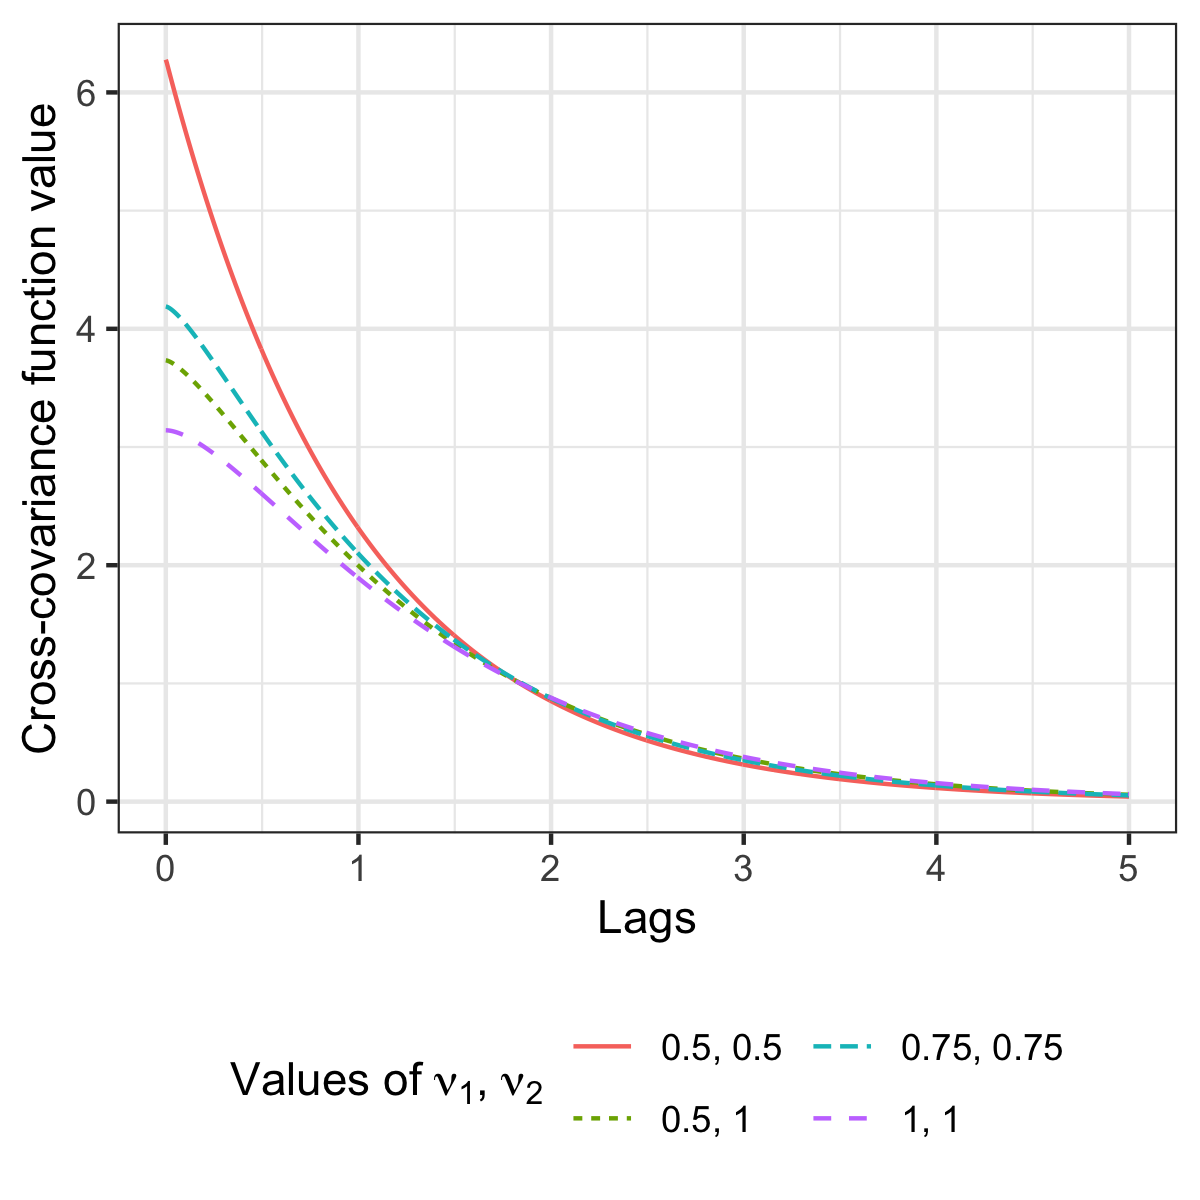
\includegraphics[scale = .15]{../symmetric_spat.png}
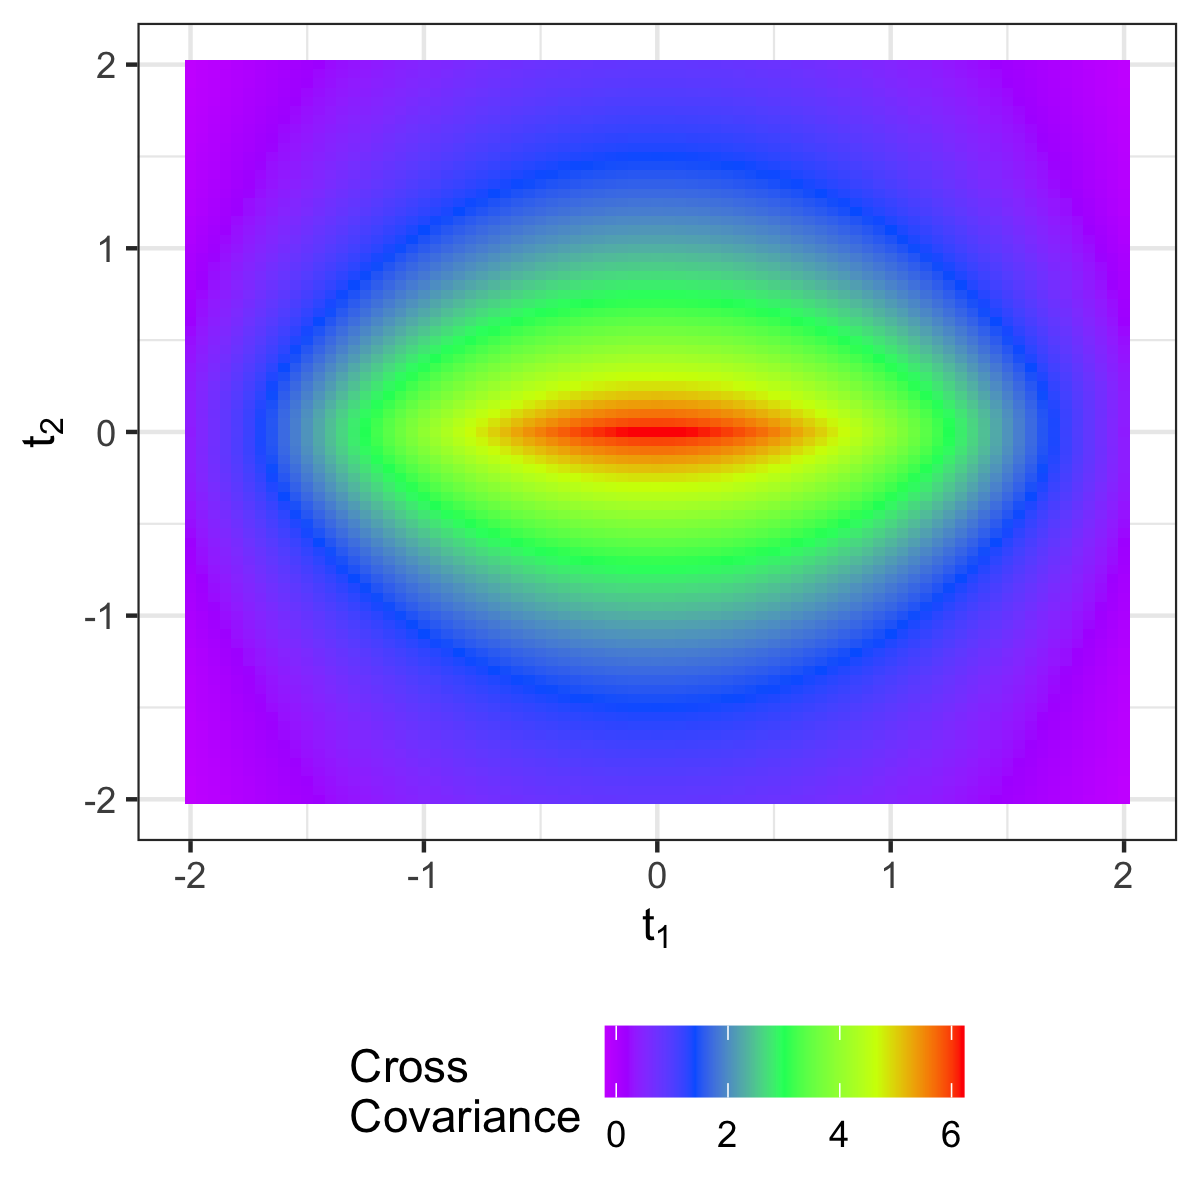
\includegraphics[scale = .15]{../asymmetric_spat_e.png}
\caption{
(Left) For $d=2$, multivariate Mat\'ern cross-covariances with $a_1 = a_2 = 1$, $E = I_2$, $\Delta_{12}(d\theta) = d\theta$, and varying values for $\nu_1$ and $\nu_2$. All except $\nu_1 = 0.5$ and $\nu_2 = 1$ correspond to a Mat\'ern covariance. (Right) For $d=2$, multivariate Mat\'ern cross-covariance with $a_1 = a_2 = 1$, $E = \textrm{diag}(1/4, 1)$, $\Delta_{12}(d\theta) = d\theta$, and $\nu_1 = \nu_2 = 0.5$.}
\label{fig:spatial1}
\end{figure}


\subsection{With varying $\Delta(d\theta)$}

Even when $\Delta$ is a constant measure, this introduces a new set of cross-covariances for any $d$. The cross-covariances can become more interesting when $\Delta(d\theta)$ is not constant but rather depends on $d\theta$. 

We first outline one particular area where the result is similar to the $d=1$ case. In particular, we let $\Delta(d\theta) = AA^* 1_{\theta_1 > 0} + \overline{AA^*}1_{\theta_1 < 0}$. In this case, $\theta_1$ is the first entry of $\theta$, and we choose this axis arbitrarily; such a formulation can be extended to the conditions of $\langle y, \theta\rangle >0$ and $<0$, and so forth for some vector $y$. Then, if $t_1 - t_2$ has first entry $0$, that is $t_1 - t_2 \in \textrm{span}\{e_2,e_3,\dots, e_d\}$ where $e_q$ is the $q$-th standard basis function, $$\int_{S_0} e^{i\langle t_1 - t_2, r\theta\rangle}\Delta(d\theta)=0,$$so that the cross-covariance is $0$, implying an axis of reflection across $e_1$. 

Alternately, when $t_1 - t_2 = ce_1$ for $c \in \mathbb{R}$, we have \begin{align*}
\int_{S_0} e^{i\langle t_1 - t_2, r\theta\rangle}\Delta(\theta)&= \int_{S_0, \theta_1 > 0}e^{ic\theta_1r}AA^* d\theta +  \int_{S_0, \theta_1 < 0}e^{ic\theta_1r}\overline{AA^*} d\theta \\
&=\textrm{Re}(AA^*)\int_{S_0}e^{ic\theta_1r} d\theta -2\textrm{Im}(AA^*) \int_{S_0, \theta_1 > 0}\sin(\theta_1 cr)d\theta, 
\end{align*}a similar breakdown in the one-variable case. 
Then, once again approaching this similarly to page 154 of \cite{stein_introduction_1975} or page 43 of \cite{stein_interpolation_2013}, we have \begin{align*}
\int_{S_0, \theta_1 > 0}\sin(\theta_1 cr)d\theta &\propto \int_0^{\pi/2}\sin(\cos(\phi) cr) \sin^{d-1}(\phi)d\phi\propto(cr)^{-(d-2)/2} H_{(d-2)/2}(cr)
\end{align*}by using standard integral representation of the Struve function $H_\nu(x)$.
% Then, by making the change of variables $\theta_1 = \cos(\phi)$ and $p = \sqrt{\theta_1^2 + \theta_2^2}$ with $d\theta_1 = -\sin(\phi) d\phi$ \begin{align*}
% \int_{S_0, \theta_1 > 0}\sin(\theta_1 r)d\theta = \int_{0}^\pi \sin(\cos(\phi) r) d\phi \propto \left\lVert t_1 - t_2\right\rVert^{-d/2 + 1/2} r^{-d/2 + 1/2} H_{d/2 - 1/2}(r\left\lVert t_1 - t_2\right\rVert)
% \end{align*}where $H_\nu(x)$ is the Stuve function (TODO: prove or point to reference). 
Then, when $\nu = \textrm{diag}(\nu_1, \nu_1)$, $E = I$, and $a =  \textrm{diag}(a_1, a_1)$,
applying 6.814 of \cite{noauthor_table_2015} to this expression, the cross-covariance in this direction is proportional to $\textrm{sign}(c)|c|^{\nu_1} \left(I_{\nu_1}(|c|) - L_{-\nu_1}(|c|)\right)$, so that it matches the $d=1$ case.
An example of this cross-covariance is plotted in Figure~\ref{fig:spatial2}.

This measure $\Delta$ offers a broad array of potential symmetries in the domain of the process. \cite{didier_domain_2018} provide more insight about the possibilities, characterizing all possible domain and range symmetries in the case $K = d = 2$. 
As one example, we plot another cross-covariance with two axes of reflection in Figure~\ref{fig:spatial2}.
%, though they only   

\begin{figure}
\centering
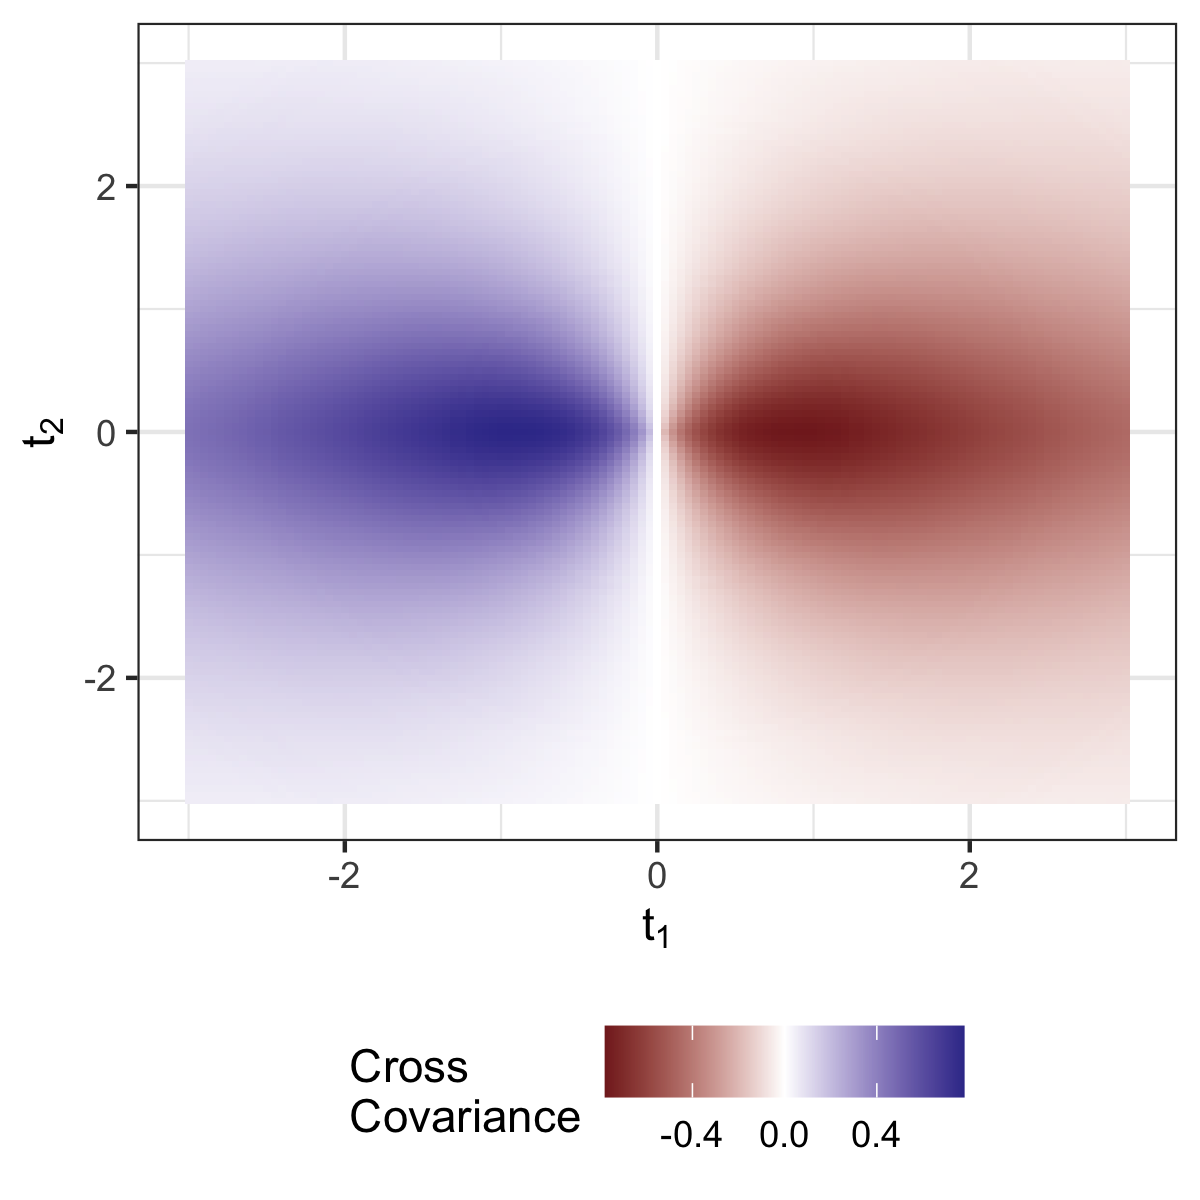
\includegraphics[scale = .15]{../asymmetric_spat.png}
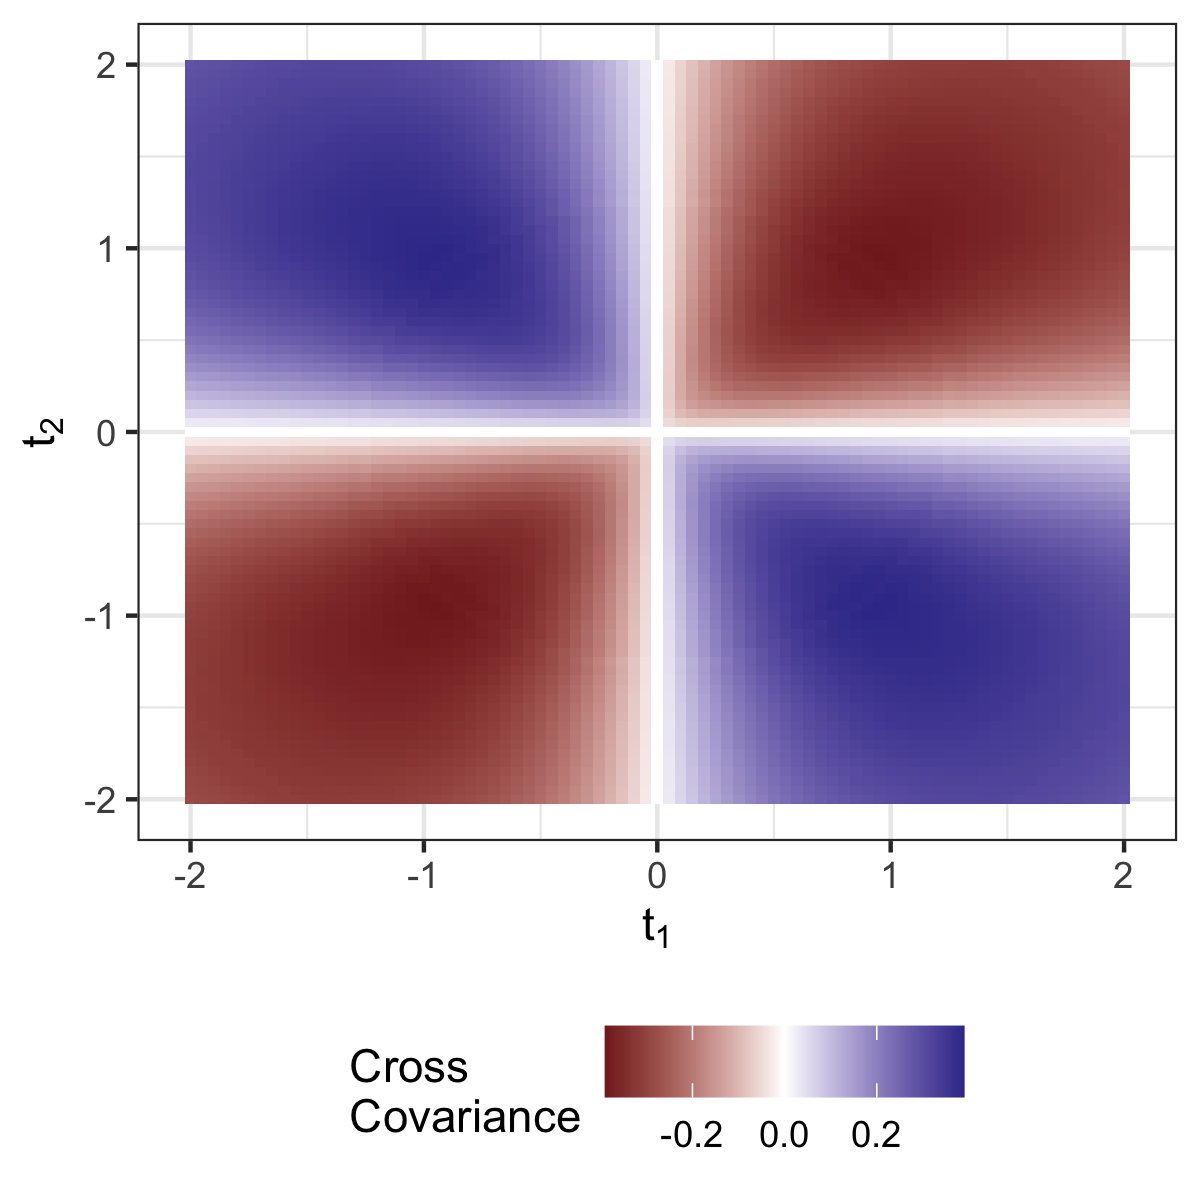
\includegraphics[scale = .15]{../asymmetric_spat_theta_weird.png}
\caption{
(Left) For $d=2$, multivariate Mat\'ern cross-covariance with $a_1 = a_2 = 1$, $E = I_2$, $\nu_1 = \nu_2 = 0.5$ and $\Delta_{12}(d\theta) = 0.3(i1_{\theta_1 > 0} - i1_{\theta_1 < 0})d\theta$.  (Right) $a_1 = a_2 = 1$, $E = I_2$, $\Delta_{12}(d\theta) = 0.3\left(1_{\textrm{sign}(\theta_1) = \textrm{sign}(\theta_2)} - 1_{\textrm{sign}(\theta_1) \neq \textrm{sign}(\theta_2)}\right) d\theta$, and $\nu_1 = \nu_2 = .5$.}
\label{fig:spatial2}
\end{figure}


\subsection{Simulation and Estimation}

Since many of the integrals presented above are not necessarily available in closed form, we approximate the integrals for the plots in this section. Futhermore, the processes can be simulated efficiently. In particular, we use the approach in \cite{emery_improved_2016} as recommended in \cite{alegria_bivariate_2021}, which uses the spectral density and a form of importance sampling to simulate the multivariate process. 

We plot simulated processes in Figure~\ref{fig:simulated_spatial}, for different $\Delta$ and $\nu$.



\begin{figure}
\centering
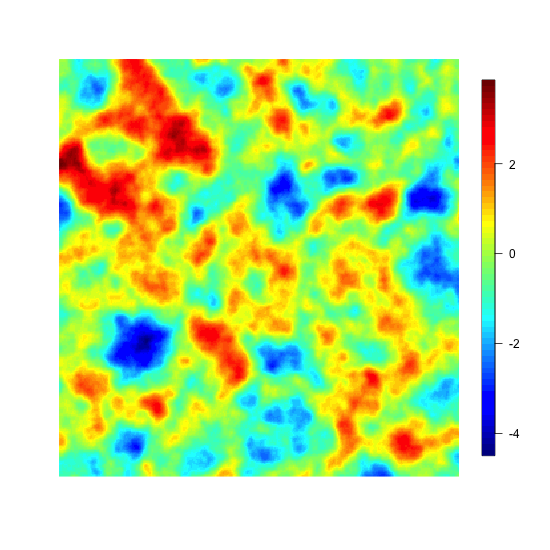
\includegraphics[scale = .35]{../simu_spatial1.png}
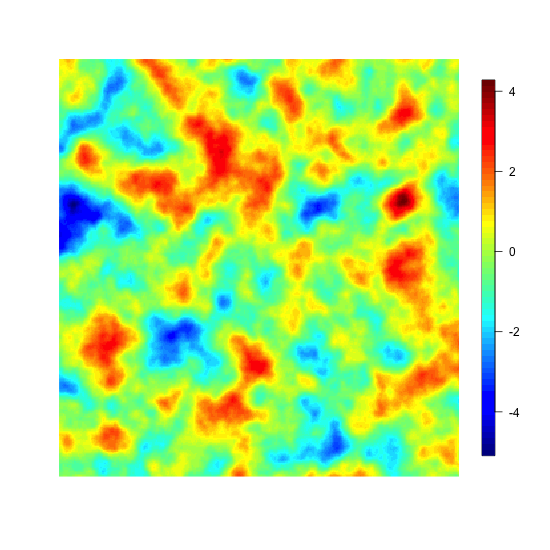
\includegraphics[scale = .35]{../simu_spatial2.png}

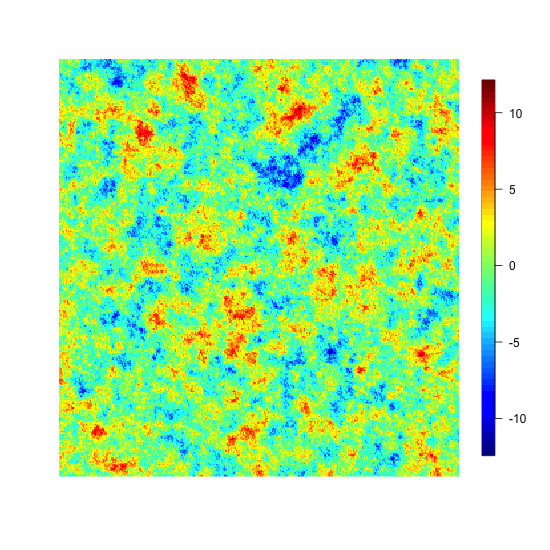
\includegraphics[scale = .35]{../simu_spatial3.png}
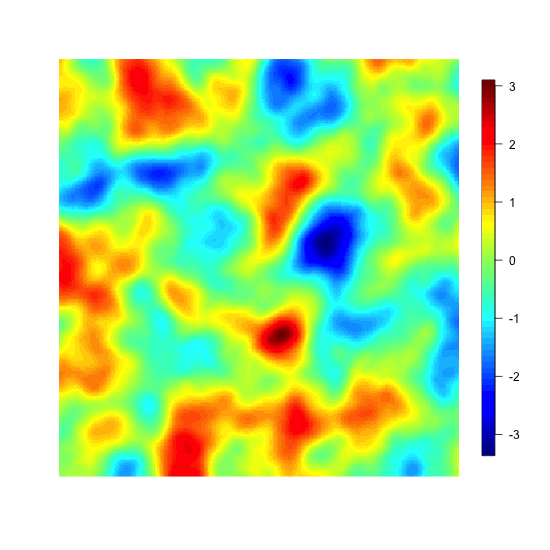
\includegraphics[scale = .35]{../simu_spatial4.png}

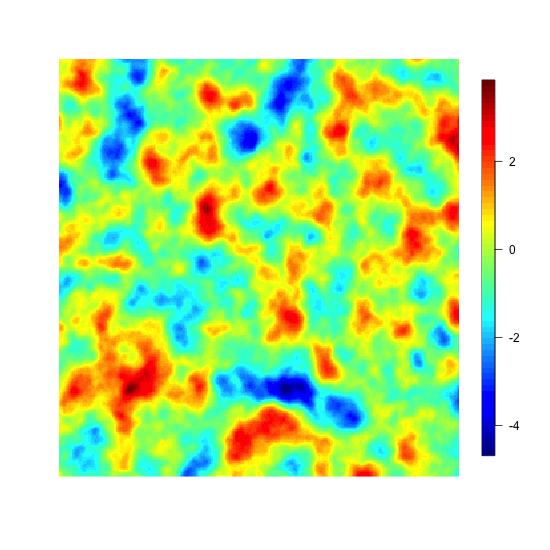
\includegraphics[scale = .35]{../simu_spatial5.png}
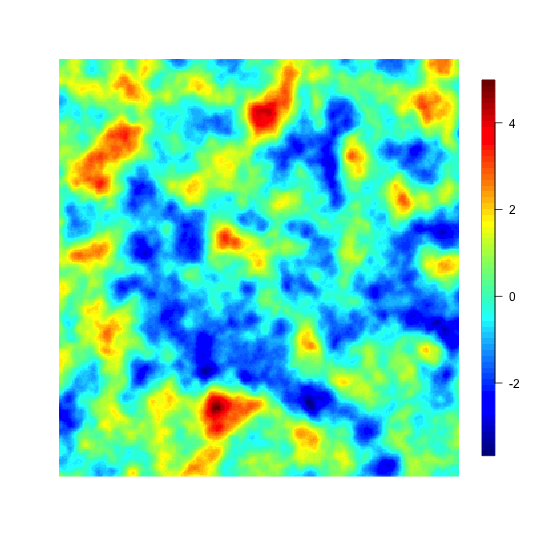
\includegraphics[scale = .35]{../simu_spatial6.png}
\caption{(Left) Process 1 (Right) Process 2, each over a grid from $0$ to $25$. (Top) One realization with $a_1 = a_2 = 1$, $\nu_1 = \nu_2 = 1.5$, $\Delta(d\theta) = \Sigma 1_{\theta_1 > 0}  +\overline{\Sigma} 1_{\theta_1 < 0}$, $\Sigma_{11} = \Sigma_{22} = 1$, $\Sigma_{12} = 0.97i$, and $E = I_2$. The second process shows some positive correlation with a left-shifted version of the first process. (Middle) The same as ``top,'' except with $\nu_1 = 0.4$ and $\nu_2 = 2.5$. (Bottom) Same as ``top,'' except with $\Delta_{12}(d\theta) = 0.97( 1_{\textrm{sign}(\theta_1) = \textrm{sign}(\theta_2)}-1_{\textrm{sign}(\theta_1) \neq \textrm{sign}(\theta_2)}) d\theta$.} %This represents strong dependence in the diagonal direction $y = -x$, but little dependence between the processes in the perpendicular direction.}
\label{fig:simulated_spatial}
\end{figure}



\section{Data Analysis}\label{sec:data_analysis}

To illustrate the use of this new multivariate Mat\'ern model, we consider a dataset that numerous other papers have considered for comparison \citep{gneiting_matern_2010,apanasovich_valid_2012, bolin_multivariate_nodate}, a set of temperature and pressure observations in the Pacific Northwest. Let $M(h; a, \nu)$ be a Mat\'ern correlation function. To fit the bivariate field, we consider the following models: (IM) univariate Mat\'ern models $M(h; a, \nu)$ fit to each processs independently; (PM) the model $\Sigma M(h; a, \nu)$ multiplied elementwise (assuming all covariances and cross-covariances have the same $a$ and $\nu$ parameter); (ParsM) the parsimonious Mat\'ern model as in \citep{gneiting_matern_2010}, where the covariance $\Sigma \begin{pmatrix}M(h; a, \nu_{11}) & M(h; a, \nu_{12}) \\ M(h; a, \nu_{12}) & M(h; a, \nu_{22})\end{pmatrix}$ where $\nu_{12} = \frac{\nu_1 + \nu_2}{2}$, (FBM) the full bivariate Mat\'ern model as in \cite{gneiting_matern_2010}.

We use the optim function with the L-BFGS-B algorithm to estimate the parameters by maximum likelihood. 

% We illustrate the use of the multivariate Matérn model on a meteorological dataset which consists of temperature and pressure observations and forecasts at 157 locations in the North American Pacific Northwest, as shown in Figure 3. The forecasts are from the GFS member of the University of Washington regional numerical weather prediction ensemble (Eckel and Mass 2005); they are valid on December 18, 2003 at 4 p.m. local time, at a forecast horizon of 48 hours. The bivariate (p = 2) spatial random field which we consider is the error field that arises as forecast minus observation. Our applied motivation lies in probabilistic weather field forecasting (Gel, Raftery, and Gneiting 2004; Berrocal, Raftery, and Gneiting 2007, 2008), which relies on the ability to fit and sample spatially correlated error fields. Here, we aim to fit a random field model for pressure and temperature errors that honors the salient features of these fields. It is customary to assume Gaussian fields with mean zero. Forecast fields are smooth, so the error fields inherit their properties from the observation


{\bf Should I make a few plots} of the d=1 imaginary entries with different scales/smoothness parameters by estimating the integral?

\section{Space-time multivariate Mat\'ern processes or lagged covariance structures}



% @article{qadir_modeling_2022,
% 	title = {Modeling and {Predicting} {Spatio}-temporal {Dynamics} of {PM}\$\_\{2.5\}\$ {Concentrations} {Through} {Time}-evolving {Covariance} {Models}},
% 	url = {http://arxiv.org/abs/2202.12121},
% 	abstract = {Fine particulate matter (PM\$\_\{2.5\}\$) has become a great concern worldwide due to its adverse health effects. PM\$\_\{2.5\}\$ concentrations typically exhibit complex spatio-temporal variations. Both the mean and the spatio-temporal dependence evolve with time due to seasonality, which makes the statistical analysis of PM\$\_\{2.5\}\$ challenging. In geostatistics, Gaussian process is a powerful tool for characterizing and predicting such spatio-temporal dynamics, for which the specification of a spatio-temporal covariance function is the key. While the extant literature offers a wide range of choices for flexible stationary spatio-temporal covariance models, the temporally evolving spatio-temporal dependence has received scant attention only. To this end, we propose a time-varying spatio-temporal covariance model for describing the time-evolving spatio-temporal dependence in PM\$\_\{2.5\}\$ concentrations. For estimation, we develop a composite likelihood-based procedure to handle large spatio-temporal datasets.The proposed model is shown to outperform traditionally used models through simulation studies in terms of predictions. We apply our model to analyze the PM\$\_\{2.5\}\$ data in the state of Oregon, US. Therein, we show that the spatial scale and smoothness exhibit periodicity. The proposed model is also shown to be beneficial over traditionally used models on this dataset for predictions.},
% 	urldate = {2022-02-25},
% 	journal = {arXiv:2202.12121 [stat]},
% 	author = {Qadir, Ghulam A. and Sun, Ying},
% 	month = feb,
% 	year = {2022},
% 	note = {arXiv: 2202.12121},
% 	file = {Qadir & Sun(2022)Modeling and Predicting Spatio-temporal Dynamics of PM\$_ 2.pdf:/Users/dyarger/Dropbox (University of Michigan)/Zotero/Qadir & Sun(2022)Modeling and Predicting Spatio-temporal Dynamics of PM\$_ 2.pdf:application/pdf},
% }



\section{Discussion}

In this work, we introduce a new class of multivariate Mat\'ern models whose tangent processes are operator fractional Brownian motion \citep[see][]{shen_tangent_2021, didier_integral_2011}. This class of models provides more flexible forms of the cross-covariance structure compared to the multivariate Mat\'ern of \cite{gneiting_matern_2010}. 
In particular, asymmetry in the cross-covariance can be modeled straightforwardly. 
Furthermore, compared to that of the multivariate Mat\'ern of \cite{gneiting_matern_2010}, there are fewer parameters, validity of the cross-covariance is given without complicated restrictions on the parameters, and the parameters succinctly represent the nature of the dependence between univariate Mat\'ern processes. 
We show that the parameters are estimable and have straightfoward interpretations, allowing one to choose the amount of flexibility in the model. 
We also provide clarity in how previous work on multivariate Mat\'ern models fit into the framework developed here. 
Under particular parameters in the time series setting of $d=1$, closed-form expressions for the cross-covariance are given.

We initially focus on the case where $d=1$; afterwards, we expand to consider spatial models for $d \geq 2$. 
In the spatial case, flexible representations of the cross covariance with respect to the domain are available. 
A fruitful area of further research would investigate the extent of the existence of closed-form spatial covariances. 
On the other hand, the flexibility of such models suggests that closed-form cross-covariances may be elusive, and the authors have explored possible approaches to no avail \citep[for example,][]{agrest_general_1971}.
To address this challenge, we demonstrate that spatial processes with these cross-covariances can be easily simulated using existing approaches for multivariate random fields, and the cross-covariance functions can be evaluated through their spectral density.
Future work could also introduce computational methodology to use the model presented here for large-scale data analysis. 

As a byproduct of the general availability of validity of the model for $K$-variate processes, we develop a multivariate-generated functional Mat\'ern model that considers the model presented here as $K \to \infty$. Further development of this model would be of theoretical and practical interest for a variety of spatial functional data analysis applications.


% The work in this paper can be extended in a variety of ways, some more straightforward than others. For example, the case where $\nu$ is diagonalizable should be relatively straightforward. In this work, we also develop a functional Mat\'ern model based on a asymptotic version of the multivariate model. 
% Further development of this model would be of theoretical and practical interest. 

% On the other hand, finding closed-form covariances for $d > 1$ or adapting it for large-scale data analysis will likely be more challenging. 
% Similarly, further development of the functional Mat\'ern model presented here would be of theoretical and practical interest. 

%Extended to when $\nu$ is diagonalizable. 




\pagebreak

\appendix

\section{Characterization of non-reversible models in $d=1$}

We now turn to the more general case where $\nu_1 - \nu_2$ is an integer and $a_1 = a_2 = 1$. This shows a partial attempt to completely characterize the multivariate Mat\'ern models when $d=1$. 

\begin{theorem}
Suppose $\nu_1 - \nu_2$ is an integer, $\textrm{Re}(\Sigma_{12}) = 0$, $\nu_1 > 0$, $\nu_2 > 0$, and $a_1 = a_2 = 1$. If $h > 0$, the cross-covariance is \begin{align*}
\textrm{Im}(\Sigma_{12}) c_\nu
(h/2)^{\nu_+-\frac12}\left(\frac{M_{\nu_-,\nu_+}(2h)}{\Gamma(1 + 2\nu_+)\Gamma(\frac12 - \nu_{1})} - \frac{ A_{\nu_-,-\nu_+}(2h)}{\Gamma(1 - 2\nu_-)\Gamma(\frac12 + \nu_{2})}\right)
\end{align*}where $M_{\mu, \kappa}(t)$ is the first Whittaker function, and $A_{\mu, \kappa}(t)$ is the generalized modified Struve function defined by \cite{babister_transcendental_1967}, and \begin{align*}
c_\nu = \frac{2\pi^2(\cos(2 \pi \nu_1) + 1)}{\Gamma(1/2 + \nu_{1})(\cos(\pi (2\nu_1 + 2\nu_2-1)) - 4\cos(2\pi \nu_1) - 3)}.
%\frac{\textrm{Im}(\Sigma_{12}) }{2\cos(\pi \nu_1)\cos(\pi \nu_2) }
\end{align*}
\end{theorem}

\begin{remark}[Implementation]\normalfont
The Whittaker function $M_{\mu, \kappa}$ are implemented in the R package \texttt{fAsianOptions} as well as Mathematica. The authors have thus far not found a proper implementation of the generalized modified Struve function $A_{\mu, \kappa}$.
\end{remark}



% As a special case where $\nu_1 = \nu_2$, we provide a simplified version of the theorem.

% \begin{remark}
% When $\nu_1 = \nu_2$, the proof is direct and the result more simple. Using \cite{noauthor_table_2015} 3.771 2, we have \begin{align*}
% \mathbb{E}\left(Y(t) Y(s)^*\right) &=-\textrm{Im}(D_{12})c_1\textrm{sign}(h)|h|^{\nu_1} \left(I_{\nu_1}(|h|) - L_{-\nu_1}(|h|)\right) 
% \end{align*}where 
% %c_1 &= \frac{2}{\sqrt{\pi}} \frac{1}{2^\nu}\cos(-\pi \nu) \Gamma(-\nu + 1/2)\\
% $c_1 =  \frac{\sqrt{\pi}}{2^{\nu_1}}\Gamma(-\nu_1 + 1/2)$, 
% $I_\nu(t)$ is the modified Bessel function of the first kind, and 
% $L_\nu(t)$ is the modified Struve function. This is only valid when $\nu_1 \neq 1/2, 3/2, \dots$. See \url{https://argo.stat.lsa.umich.edu/shiny/ShinyApps/multivariate_matern/} to see various plots of the covariances and cross covariances.
% \begin{figure}
% \centering
% 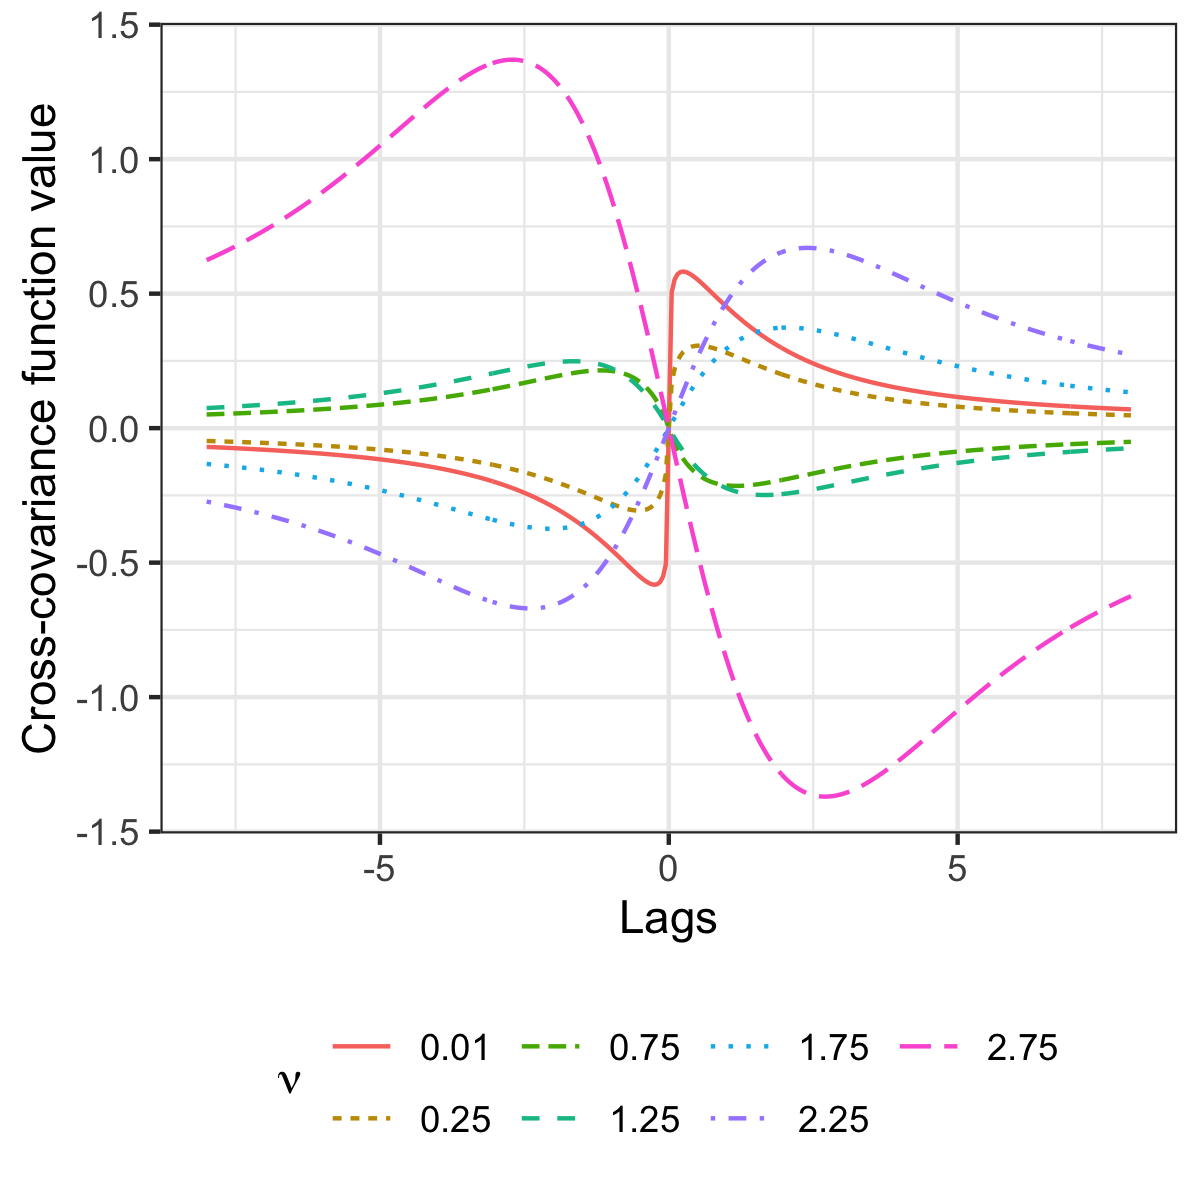
\includegraphics[scale = .08]{../example_fun.png}
% \caption{The function $\textrm{sign}(h)|h|^{\nu_1} \left(I_{\nu_1}(|h|) - L_{-\nu_1}(|h|)\right)$ for various $\nu_1$.}
% \end{figure}
% \end{remark}
\begin{proof}

Now, we must deal with the general form (\ref{impart2}). Note that we can write this term as \begin{align*}
2\textrm{Im}(\Sigma_{12}) \textrm{Re}(X(\nu_{1}, \nu_{2};h))
\end{align*}where $h = t-s$ and \begin{align*}
X(\nu_{1}, \nu_{2};h) &:= i \int_0^\infty e^{ihx}(1 + ix)^{-\nu_1 - 1/2}(1 - ix)^{-\nu_2 - 1/2} dx.
\end{align*}This follows by considering the conjugate of $X(\nu_{1}, \nu_{2};h)$ and adjusting the limits of integration. 

Referring to Equation 4.44 of \cite{babister_transcendental_1967}, we define \begin{align*}
Z(a,c;z) &= ie^{-i\pi(a - c/2)}(e^{2\pi i a}- 2 + e^{-2\pi i(c-a)})\int_0^\infty e^{isz}\left(s-\frac{i}{2}\right)^{a-1}\left(s + \frac{i}{2}\right)^{c-a-1} ds 
\end{align*}and aim to write $X$ in terms of $Z$:
\begin{align*}
X(\nu_1, \nu_2; h) &= i\int_0^\infty e^{ihx} (1 + ix)^{-\nu_1 - 1/2}(1 -ix)^{-\nu_2-1/2} dx \\
&=i(-i)^{-\nu_1 - 1/2}i^{-\nu_2 - 1/2} \int_0^\infty e^{ihx}(x-i)^{-\nu_1 - 1/2} (x + i)^{-\nu_2 - 1/2} dx \\
&=i(-i)^{-\nu_1 - 1/2}i^{-\nu_2 - 1/2} 2^{-\nu_1 - \nu_2 - 1}\int_0^\infty e^{ihx}\left(\frac{x}{2}-\frac{i}{2}\right)^{-\nu_1 - 1/2} \left(\frac{x}{2} + \frac{i}{2}\right)^{-\nu_2 - 1/2} dx.\end{align*} Then, by making the change of variables $s = x/2$, we have
\begin{align*}
X(\nu_1, \nu_2; h)&=i(-i)^{-\nu_1 - 1/2}i^{-\nu_2 - 1/2} 2^{-\nu_1 - \nu_2}\int_0^\infty e^{ih2s}\left(s-\frac{i}{2}\right)^{-\nu_1 - 1/2} \left(s + \frac{i}{2}\right)^{-\nu_2 - 1/2} ds\\
&=\frac{i(-i)^{-\nu_1 - 1/2}i^{-\nu_2 - 1/2} 2^{-\nu_1 - \nu_2}Z(1/2 - \nu_1, 1- \nu_1 - \nu_2; 2h)}{ie^{-i \pi (1/2)(-\nu_1 +\nu_2)}(e^{2\pi i (1/2 - \nu_1)} - 2+ e^{-2\pi i (1/2 - \nu_2)}) }\end{align*}by substituting the expression for $Z(a,c;h)$. Finally, evaluation of the complex constant through Wolfram Alpha yields \begin{align*}
X(\nu_1, \nu_2; h) &= \frac{\cos(2 \pi \nu_1) + \cos(2\pi\nu_2) + 2 +i (\sin(2\pi \nu_1) - \sin(2\pi \nu_2))}{2\cos(\pi (4\nu_+-1)) - 4\cos(2\pi \nu_1) - 4 \cos(2\pi \nu_2) - 6}2^{-\nu_1 - \nu_2}Z(1/2 - \nu_1, 1- \nu_1 - \nu_2; 2h),
\end{align*}recalling the definitions $\nu_+ = (\nu_1 + \nu_2)/2$ and $\nu_- = (\nu_1 - \nu_2)/2$. Now, assume that $\nu_1 - \nu_2$ is an integer, which ensures that the imaginary part in the numerator is zero.
%Now, we have to make a leap that $\textrm{Re}(X(\nu_1, \nu_2; h)) = Z(1/2 - \nu_1, 1- \nu_1 - \nu_2; 2h)$ up to a real-valued constant. If that is the case (but requires more work), we can derive the functional form. I do think we are going in the right direction, but more details need to be worked out. If we take this to be true, 
Then, according to Equation 4.45 of \cite{babister_transcendental_1967}, for $h > 0$, \begin{align*}
\textrm{Re}(Z(1/2 - \nu_{1},1 -2\nu_+;2h))% &= \frac{2\pi^2e^{-z/2}}{\Gamma(1-a)}\left(\frac{\Omega(a,c;z)}{\Gamma(c)\Gamma(1+a-c)} - \frac{1}{\Gamma(2-c)\Gamma(a)}\overline{\Phi}(a,c;z)\right)\\
&= \frac{2\pi^2e^{-h}}{\Gamma(\frac12 + \nu_{1})}\left(\frac{\Omega(\frac12 - \nu_{1},1 - 2\nu_+;2h)}{\Gamma(1 -2\nu_+)\Gamma(\frac12 + \nu_{2})} - \frac{\overline{\Phi}(\frac12 - \nu_{1},1 - 2\nu_{+};2h)}{\Gamma(1 + 2\nu_+)\Gamma(\frac12 - \nu_{1})}\right)
\end{align*}where $\Omega$ is the generalized modified Struve function defined in Equation 4.30 of \cite{babister_transcendental_1967}, and $\overline{\Phi}$ is the confluent hypergeometric function defined in Equation 4.7 of \cite{babister_transcendental_1967}. Notably, these reduce to other functions for certain values of the parameters (see Equations 5.11 and 5.16 of the same text), which we define here: \begin{align*}
M_{\kappa,- \mu}(z) &=  e^{-z/2}z^{1/2 +\mu}\overline{\Phi}(1/2- \kappa + \mu, 1 + 2\mu; z)\\
A_{\kappa, \mu}(z) &= e^{-z/2}z^{1/2 + \mu}\Omega(1/2- \kappa + \mu, 1 + 2\mu; z)
\end{align*}We refer to $M_{\kappa, \mu}$ as the Whittaker function of the first kind, and $A_{\kappa, \mu}$ as (another) generalized modified struve function \citep{babister_transcendental_1967}. Notably (as in Equations 5.12 and 5.19), for certain values these reduce further to the Bessel function of the second kind ($I_\mu$) and the modified Struve function $L_\mu$:\begin{align*}
M_{0,\mu}(z) &= 2^{2\mu}\Gamma(\mu + 1)z^{1/2}I_\mu(z/2)\\
A_{0,\mu}(z) &= 2^{2\mu}\Gamma(\mu + 1)z^{1/2}L_\mu(z/2).
\end{align*}

Using the definitions of $M_{\kappa, \mu}$ and $A_{\kappa, \mu}$ above with $\kappa = \nu_-$ and $\mu = -\nu_+$, we write\begin{align*}
\textrm{Re}(Z(1/2 - \nu_{1},1 - 2\nu_+;2h)) &= \frac{2\pi^2(2h)^{\nu_+-\frac12}}{\Gamma(\frac12 + \nu_{1})}\left(\frac{ A_{\nu_-,-\nu_+}(2h)}{\Gamma(1 - 2\nu_+)\Gamma(\frac12 + \nu_{2})} - \frac{M_{\nu_-,\nu_+}(2h)}{\Gamma(1 + 2\nu_+)\Gamma(\frac12 - \nu_{1})}\right).
\end{align*}Thus, when the smoothness of the two processes are the same, we will revert to the more familiar $I_\nu$ and $L_\nu$ as in Theorem \ref{thm:im_ent} from the functions $M_{\kappa, \nu}(z)$ and $A_{\kappa, \nu}(z)$, respectively.

Thus, piecing it all together, the cross-covariance is \begin{align*}
 \frac{(\cos(2 \pi \nu_1) + 1)\textrm{Im}(\Sigma_{12})}{\cos(\pi (4\nu_+-1)) - 4\cos(2\pi \nu_1) - 3}
%\frac{\textrm{Im}(\Sigma_{12}) }{2\cos(\pi \nu_1)\cos(\pi \nu_2) }
\frac{2\pi^2(h/2)^{\nu_+-\frac12}}{\Gamma(\frac12 + \nu_{1})}\left(\frac{M_{\nu_-,\nu_+}(2h)}{\Gamma(1 + 2\nu_+)\Gamma(\frac12 - \nu_{1})} - \frac{ A_{\nu_-,-\nu_+}(2h)}{\Gamma(1 - 2\nu_-)\Gamma(\frac12 + \nu_{2})}\right)
\end{align*}since  $\cos(2\pi\nu_2) = \cos(2\pi\nu_1)$ when $\nu_2 - \nu_1$ is an integer.

% The above analysis was done assuming $h > 0$. When $h < 0$, applying change of variables in $X(\nu_1, \nu_2;h)$ yields \begin{align*}
%  \frac{(\cos(2 \pi \nu_1) + 1)\textrm{Im}(\Sigma_{12})}{\cos(\pi (4\nu_+-1)) - 4\cos(2\pi \nu_1) - 3}
% %\frac{\textrm{Im}(\Sigma_{12}) }{2\cos(\pi \nu_1)\cos(\pi \nu_2) }
% \frac{2\pi^2(h/2)^{\nu_+-\frac12}}{\Gamma(1/2 + \nu_{1})}\left(\frac{M_{\nu_-,\nu_+}(2h)}{\Gamma(1 + 2\nu_+)\Gamma(\frac12 - \nu_{1})} - \frac{ A_{\nu_-,-\nu_+}(2h)}{\Gamma(1 - 2\nu_-)\Gamma(\frac12 + \nu_{2})}\right)
% \end{align*}for $h$ negative.
\end{proof}





\bibliography{multivariate_matern}

\end{document}



%It's possible to compute using \ref{pandey_numerical_2010}, \cite{cree_algorithms_1993}, \cite{knockaert_fast_2000},\cite{lucas_evaluating_1995}. But maybe focus on \cite{emery_improved_2016} for computing it. 


% 
% Note Note Note: The eigenvalue of $\nu - d I /2$ cannot be $0$, this may be why things don't work out for $\nu_1 + \nu_2$ an integer for real entries, and $\nu_1=\nu_2 = 1/2$ for imaginary entries, etc. 
%   \begin{equation}
%    Y(t):= \int_{0}^\infty \int_{S_0} (e^{i\langle t,r^{E^*}\theta\rangle}-1) r^{-H-1/2} B_{H,\Delta}(dr,d\theta),
%    \end{equation} where $\mathbb{E}(B_{H, \Delta} B_{H,\Delta}^*) = \Delta(d\theta)dr$. When $d=1$, OFBM takes $\Delta(d\theta) = AA^* 1_{d\theta = 1} + \overline{AA^*}1_{d\theta = -1} = AA^* 1_{x > 0} + \overline{AA}^*1_{x < 0}$. Note that $\theta \in \{-1,1,0\}$ because we are in the one dimensional case. 
%    
%    Step 1: Assume $\Delta$ is uniform, adjust integral to something multivariate Mat\'ern like, see what happens:
%     \begin{equation}
%    Y(t):= \int_{0}^\infty \int_{S_0} e^{i\langle t,r^{E^*}\theta\rangle} (a + ir)^{-H-1/2} B_{H,\Delta}(dr,d\theta),
%    \end{equation}
%    
%    By the covariance expression, it is \begin{equation}
%    \int_0^\infty \int_{S_0} e^{i\langle h, r^{E^*}\theta\rangle} (a + ir)^{-H-1/2}\Delta(d\theta) ((a + ir)^{-H-1/2})^* dr 
%    \end{equation}
%    
%    Letting $E =I$ and $\Delta(d\theta) = AA^*$, we get something like \begin{equation}
%    \int_0^\infty  e^{i\langle h, rI\rangle} (a + ir)^{-H-1/2}AA^* (a - ir)^{-H-1/2} dr 
%    \end{equation}This looks the same as the Whittaker function but is only integrated from $0$ to $\infty$.
%    
%    Step 2: Assume 
% 
%    Inspired by these results and the fact that operator fBm's can arise as tangent processes for stationary $\R^K$-valued models (under operator normalization), we would like to introduce an extension of the Mat\'ern model. This extension can be considered as {\em canonical} or {\em complete}, if its tangent processes can realize all possible operator fBm models. To this end, consider the process
%    \begin{equation}\label{e:o-Matern}
%    Y(t):= \int_{0}^\infty \int_{S_0} e^{i\langle t,r^{E^*}\theta\rangle}-1 ( (a+ix)^{-\nu -1/2}A 1_{\{x>0\}} + (a+ix)^{-\nu - 1/2}\overline{A}1_{\{x<0\}}) \tilde B(dx),
%    \end{equation}where $a$ and $\nu$ are $K\times K$ real-valued matrices. Here, to avoid confusion with matrix notation, we note that the matrix $(a + i x)^{-\nu - 1/2}$ has $j$, $k$ entry $(a_{jk} + ix)^{-\nu_{jk}-1_{j = k}1/2}$. The matrix $\nu$ will essentially correspond to the operator $H$ of the tangent operator fBm process associated with the above model. Due to Bochner's Theorem \citep{stein_interpolation_2013} and its extension to multivariate processes as Cramer's Theorem \citep{genton_cross-covariance_2015}, \eqref{e:o-Matern} results in a process with a valid positive-definite covariance function. 

% Thus far, we have considered only the time series setting, that is, when $d=1$. The reaches of such a model are limited, and we want to explore the space of spatial processes. When $d=2, 3, \dots$, such processes are more complicated, and closed-form solutions are elusive. In the following, we demonstrate our work in developing such processes. 
% 
% Let $ \vlen, \vint$ be vectors in $\mathbb{R}^d$. Let $\vpla$ be a vector in $\mathbb{R}^d$ that describes the plane through the origin for which the non-reversibility is reflected, defined by all $\vint$ such that $\vpla^\top \vint = 0$. Finally, define $\left\lVert \vint \right\rVert_*  =\textrm{sign}(\vint^\top \vpla) \left\lVert \vint \right\rVert$. We want to consider the covariance of \begin{align*}
% C(\boldsymbol{0}, \boldsymbol{h}) &= \int_{\mathbb{R}^d} e^{i \vint^\top \vlen} (a_1 + i \left\lVert \vint \right\rVert_* )^{-\nu_1- \frac{d}{2}}(a_2 - i \left\lVert \vint \right\rVert_* )^{-\nu_2- \frac{d}{2}} \left(\Sigma 1_{\vpla^\top \vint > 0} + \overline{\Sigma} 1_{\vpla^\top\vint < 0}\right) d\vint.% \\
% %&=\int_{\mathbb{R}^d} e^{i \vint^\top \vlen }(1 + \vint^\top \vint)^{-\nu- \frac{d}{2}} \left((R + iM)1_{\{\vpla^\top\vint > 0\}} + (R - iM) 1_{\{\vpla^\top\vint < 0\}}\right) d\vint 
% \end{align*}We motivate this so that when $d=1$, we take $\vpla = 1$, so that this reduces to \begin{align*}
% C(0,h) &= \int_{\mathbb{R}} e^{i xh} (a_1 + ix)^{-\nu_1- \frac{1}{2}}(a_2 - i x)^{-\nu_2- \frac{1}{2}} \left(\Sigma 1_{x > 0} + \overline{\Sigma} 1_{x < 0}\right) dx,
% \end{align*}the same model we consider in previous sections. To further describe this model, note how the $k$-th component has spectral density $(AA^*)_{kk}(a_k^2 + \left\lVert \boldsymbol{x}\right\rVert^2)^{-\nu_k - d/2}$, so that the marginal processes are once again Mat\'ern. 
% 
% As before, we first focus on the case where $\Sigma_{12}$ is real. 
% 
% \subsection{Spatial covariance with real entries}
% 
% Assuming that $\textrm{Im}(\Sigma_{12}) = 0$, this reduces to \begin{align*}
% C(\boldsymbol{0}, \boldsymbol{h})&=\textrm{Re}(\Sigma_{12})\int_{\mathbb{R}^d}\cos(\vint^\top \boldsymbol{h}) (1 + i \left\lVert \vint \right\rVert_* )^{-\nu_1- \frac{d}{2}}(1 - i \left\lVert \vint \right\rVert_* )^{-\nu_2- \frac{d}{2}} d\vint 
% \end{align*}
% 
% We first consider $d=2$. Note that $\vint^\top \boldsymbol{h} = r \left\lVert \boldsymbol{h}\right\rVert \cos(\theta)$ where $\theta$ is the angle between $\vint$ and $\boldsymbol{h}$ and $r = \left\lVert \vint \right\rVert$.
% Switching to these coordinates, we have \begin{align*}
% C(\boldsymbol{0}, \boldsymbol{h})&=\textrm{Re}(\Sigma_{12})\int_0^{\pi}\int_{-\infty}^\infty \cos(r\hh\cos(\theta)) (1 + ir)^{-\nu_1- 1}(1 - ir )^{-\nu_2- 1} rdr d\theta
% \end{align*}
% 
% 
% 
% We first switch to a form of $d$-dimensional spherical coordinates, inspired by a similar approach on page 43 of \cite{stein_interpolation_2013}. Note that $\vint^\top \boldsymbol{h} = r \left\lVert \boldsymbol{h}\right\rVert \cos(\theta)$ where $\theta$ is the angle between $\vint$ and $\boldsymbol{h}$ and $r = \left\lVert \vint \right\rVert$. Using these coordinates, note that the integral depends only on $r$ and $\theta$, and by integrating the other $d-2$ dimensions with volume transformation $r^{d-1}\sin^{d-2}(\theta)$, we have \begin{align*}
% C(\boldsymbol{0}, \boldsymbol{h})&=\textrm{Re}(\Sigma_{12})\int_0^{\pi}\int_0^\infty \cos(r\hh\cos(\theta)) (1 + ir)^{-\nu_1- \frac{d}{2}}(1 - ir )^{-\nu_2- \frac{d}{2}} \sin(\theta)^{d-2} r^{d-1}dr d\theta. \end{align*}Then, because $$J_\nu(z) = \frac{(\frac{z}{2})^\nu}{\sqrt{\pi}\Gamma(\nu + 1/2)} \int_0^\pi \cos(z\cos(\theta)) \sin^{2\nu}(\theta) d\theta$$ in 10.9.4 of \cite{NIST:DLMF}, we can write
% \begin{align*}
% C(\boldsymbol{0}, \boldsymbol{h})&=\textrm{Re}(\Sigma_{12})\int_0^\infty J_{(d-2)/2}(r\hh)\frac{\sqrt{\pi}\Gamma(d/2)}{(r\hh)^{(d-2)/2}}(1 + ir)^{-\nu_1- \frac{d}{2}}(1 - ir )^{-\nu_2- \frac{d}{2}} r^{d-1}dr \\
% &=\textrm{Re}(\Sigma_{12})\frac{\sqrt{\pi}\Gamma(d/2)}{\hh^{(d-2)/2}}\int_0^\infty J_{(d-2)/2}(r\hh)(1 + ir)^{-\nu_1- \frac{d}{2}}(1 - ir )^{-\nu_2- \frac{d}{2}} rdr.
% \end{align*} The sign term determines if the angle between $\boldsymbol{h}$ and $\boldsymbol{a}$ is less than or greater than $\pi/2$ degrees. Also, we here use the facts that \begin{align*}
% J_\nu(x) = \frac{(z/2)^\nu}{\sqrt{\pi}\Gamma(\nu + 1/2)}\int_0^\pi\cos(x\cos\theta)(\sin\theta)^{2\nu}d\theta
% \end{align*}


% \subsection{Spatial covariance with imaginary entries}
% 
% 
% We first aim to simplify this expression. In the spatial case, we see a similar decomposition into parts involving $\textrm{Re}(\Sigma_{12})$ and $\textrm{Im}(\Sigma_{12})$. By switching to polar coordinates (see Section \ref{sec:spat_details}), we argue below that the cross covariance reduces to \begin{align*}
% C(\boldsymbol{0}, \boldsymbol{h})_{12}&=\textrm{Re}(\Sigma_{12})\frac{\sqrt{\pi}\Gamma(d/2)}{\hh^{(d-2)/2}}\int_{-\infty}^\infty J_{(d-2)/2}(r\hh)(a_1 + ir)^{-\nu_1- \frac{d}{2}}(a_2 - ir )^{-\nu_2- \frac{d}{2}} |r|dr \\
% & \ \ \ \ \ -2\textrm{Im}(\Sigma_{12}) c_1\frac{\sqrt{\pi}\Gamma(d/2)}{\hh^{(d-2)/2}}\int_0^\infty H_{(d-2)/2}(c,r\hh)(a_1 + ir)^{-\nu_1- \frac{d}{2}}(a_2 - ir )^{-\nu_2- \frac{d}{2}} rdr
% \end{align*}where $J_\nu$ is the Bessel function, $H_\nu$ is the incomplete Struve function of \cite{agrest_general_1971}, and $c$ is the angle that $\boldsymbol{h}$ makes with $\boldsymbol{a}$.
% 
% Note that \begin{align*}
% \int_{-\infty}^\infty J_0(hx)(1 + ix)^{-1}(1-ix)^{-1} dx = \pi(I_0(h) - L_0(h))
% \end{align*}for $h > 0$. 
% 
% \begin{figure}
% \centering
% 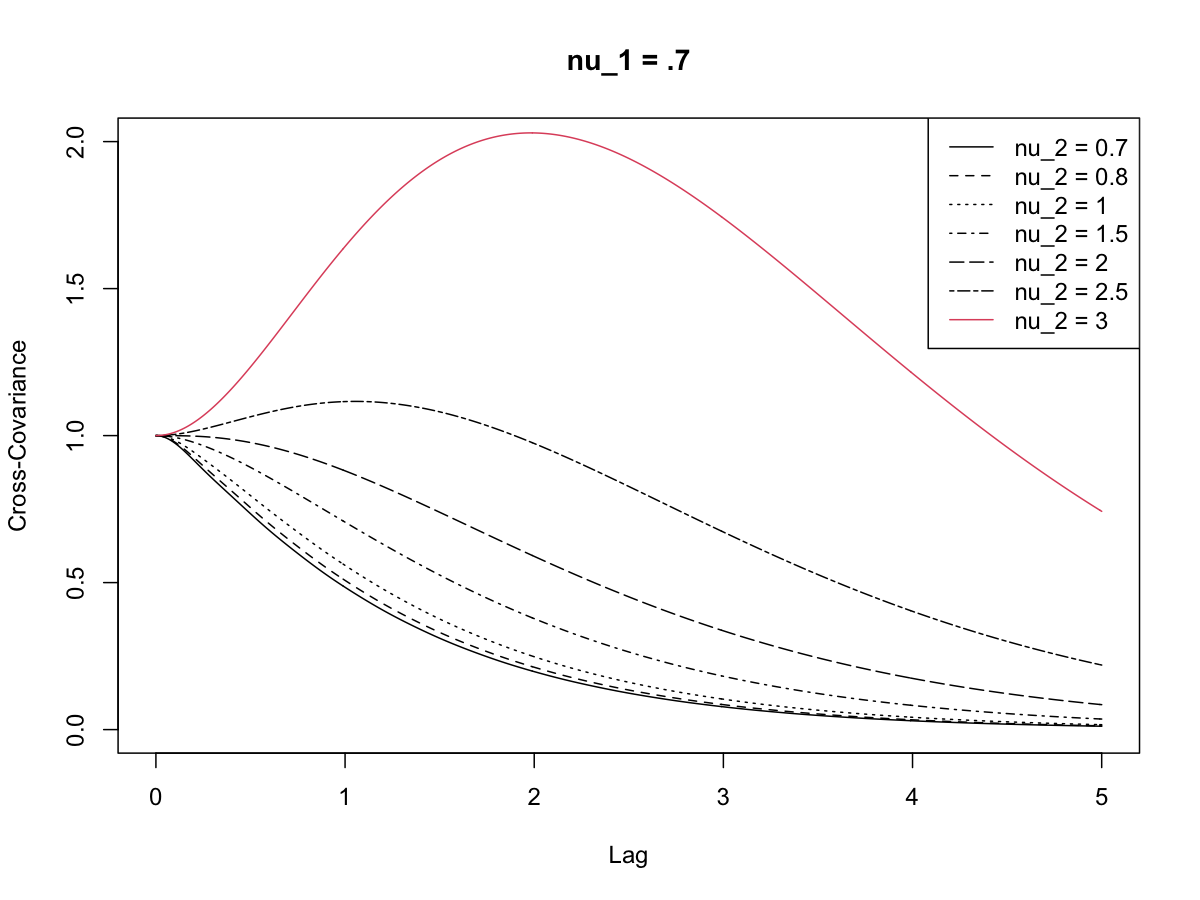
\includegraphics[scale = .2]{../d_2_ccov.png}
% 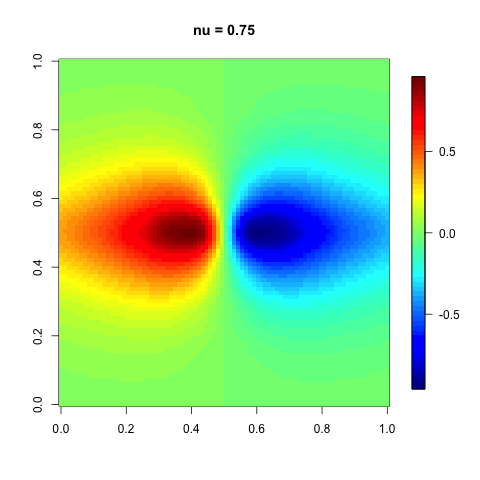
\includegraphics[scale = .45]{../images/nu0_75.png}
% \caption{(Left) Cross-covariance functions with $d=2$ for different $\nu_2$ values. This allows the maximum of the cross covariance to not be at $0$. (Right) Asymmetric part of cross-covariance for $d=2$ and $\nu_1 = \nu_2 = 0.75$. }\label{spatial}
% \end{figure}
% 
% \begin{remark}
% Note that if $\textrm{Im}(\Sigma_{12}) = 0$ and $d = 2$, then the cross-covariance is symmetric because $J_{\nu}(z)$ is symmetric for $\nu$ even. This case is plotted for varying $\nu_2$ in Figure \ref{spatial} (left) by approximating the integral. Alternately, if one supposes that $R$ is diagonal, then when $d=2$, $a = (1,0)$, then the asymmetric part of the integral is approximated and plotted in Figure \ref{spatial} for $\nu_1 = \nu_2 = 0.75$.
% \end{remark}
% 
% \begin{remark}
% If one assumes $\nu_1 = \nu_2$, the cross-covariance looks like the $d=1$ case. Namely, the first part is a standard Mat\'ern covariance, while the second part is like the 1-d case.
% \end{remark}

% \begin{proposition}
% In $d=2$, the process is time-reversible iff $\textrm{Im}(D_{12}) = 0$.
% \end{proposition}


% \subsection{Mathematical details in the spatial case}\label{sec:spat_details}
% 
% Here, we give the mathematical details.
% 
% 
% 
% Finally, define $\left\lVert \vint \right\rVert_*  =\textrm{sign}(\vint^\top \vlen) \left\lVert \vint \right\rVert$. We want to consider the covariance of \begin{align*}
% C(\boldsymbol{0}, \boldsymbol{h}) &= \int_{\mathbb{R}^d} e^{i \vint^\top \vlen} (1 + i \left\lVert \vint \right\rVert_* )^{-\nu_1- \frac{d}{2}}(1 - i \left\lVert \vint \right\rVert_* )^{-\nu_2- \frac{d}{2}} \left(AA^* 1_{\{\vpla^\top \vint > 0\}} + \overline{AA^*} 1_{\{\vpla^\top\vint < 0\}}\right) d\vint.% \\
% %&=\int_{\mathbb{R}^d} e^{i \vint^\top \vlen }(1 + \vint^\top \vint)^{-\nu- \frac{d}{2}} \left((R + iM)1_{\{\vpla^\top\vint > 0\}} + (R - iM) 1_{\{\vpla^\top\vint < 0\}}\right) d\vint 
% \end{align*}We motivate this so that when $d=1$, this reduces to the developed model in this paper.
% Plugging in $AA^* = R + iM$ gives
% \begin{align*}
% C(\boldsymbol{0}, \boldsymbol{h})&=\int_{\mathbb{R}^d} e^{i \vint^\top \boldsymbol{h}} (1 + i \left\lVert \vint \right\rVert_* )^{-\nu_1- \frac{d}{2}}(1 - i \left\lVert \vint \right\rVert_* )^{-\nu_2- \frac{d}{2}} \left(R + iM1_{\{\vpla^\top\vint > 0\}}  - iM1_{\{\vpla^\top\vint < 0\}}\right) d\vint\end{align*}
% and by breaking up the integral we have
% \begin{align*}
% C(\boldsymbol{0}, \boldsymbol{h})%&=\int_{\mathbb{R}^d} (\cos(\vint^\top \boldsymbol{h}) + i\sin(\vint^\top \boldsymbol{h}))(1 + \vint^\top \vint)^{-\nu- \frac{d}{2}} \left(R + iM1_{\{\vint > 0\}}  - iM1_{\{\vint < 0\}}\right) d\vint \\
% &=\int_{\mathbb{R}^d}\cos(\vint^\top \boldsymbol{h}) (1 + i \left\lVert \vint \right\rVert_* )^{-\nu_1- \frac{d}{2}}(1 - i \left\lVert \vint \right\rVert_* )^{-\nu_2- \frac{d}{2}}\left(R + iM1_{\{\vpla^\top\vint > 0\}}  - iM1_{\{\vpla^\top\vint < 0\}}\right) d\vint \\
% &\ \ \ \ \ \ +i\int_{\mathbb{R}^d}\sin(\vint^\top \boldsymbol{h}) (1 + i \left\lVert \vint \right\rVert_* )^{-\nu_1- \frac{d}{2}}(1 - i \left\lVert \vint \right\rVert_* )^{-\nu_2- \frac{d}{2}} \left(R + iM1_{\{\vpla^\top\vint > 0\}}  - iM1_{\{\vpla^\top\vint < 0\}}\right) d\vint.\end{align*}
% Using the even and odd properties of the cosine and sine functions, respectively, gives
% \begin{align*}
% C(\boldsymbol{0}, \boldsymbol{h})&=R\int_{\mathbb{R}^d}\cos(\vint^\top \boldsymbol{h}) (1 + i \left\lVert \vint \right\rVert_* )^{-\nu_1- \frac{d}{2}}(1 - i \left\lVert \vint \right\rVert_* )^{-\nu_2- \frac{d}{2}} d\vint \\
% & \ \ \ \ \ + i^2M\int_{\mathbb{R}^d}\sin(\vint^\top \boldsymbol{h}) (1 + i \left\lVert \vint \right\rVert_* )^{-\nu_1- \frac{d}{2}}(1 - i \left\lVert \vint \right\rVert_* )^{-\nu_2- \frac{d}{2}} \left(1_{\{\vpla^\top\vint > 0\}}  - 1_{\{\vpla^\top\vint < 0\}}\right) d\vint \\
% &=R\int_{\mathbb{R}^d}\cos(\vint^\top \boldsymbol{h}) (1 + i \left\lVert \vint \right\rVert_* )^{-\nu_1- \frac{d}{2}}(1 - i \left\lVert \vint \right\rVert_* )^{-\nu_2- \frac{d}{2}} d\vint \\
% & \ \ \ \ \ -2M\int_{\vint | \vpla^\top\vint > 0}\sin(\vint^\top \boldsymbol{h}) (1 + i \left\lVert \vint \right\rVert_* )^{-\nu_1- \frac{d}{2}}(1 - i \left\lVert \vint \right\rVert_* )^{-\nu_2- \frac{d}{2}} d\vint .
% \end{align*}
% 
% We first switch to a form of $d$-dimensional spherical coordinates. A similar approach is done in Stein (1999) page 43. Note that $\vint^\top \boldsymbol{h} = r \left\lVert \boldsymbol{h}\right\rVert \cos(\theta)$ where $\theta$ is the angle between $\vint$ and $\boldsymbol{h}$ and $r = \left\lVert \vint \right\rVert$. Using these coordinates, note that the integral depends only on $r$ and $\theta$, and by integrating the other $d-2$ dimensions with volume transformation $r^{d-1}\sin^{d-2}(\theta)$, we have \begin{align*}
% C(\boldsymbol{0}, \boldsymbol{h})&=R\int_0^{2\pi}\int_0^\infty \cos(r\hh\cos(\theta)) (1 + ir)^{-\nu_1- \frac{d}{2}}(1 - ir )^{-\nu_2- \frac{d}{2}} \sin(\theta)^{d-2} r^{d-1}dr d\theta \\
% & \ \ \ \ \ -2M \int_{-\pi+c}^c\int_0^\infty \sin(r\hh\cos(\theta)) (1 + ir)^{-\nu_1- \frac{d}{2}}(1 - ir )^{-\nu_2- \frac{d}{2}} \sin(\theta)^{d-2} r^{d-1}dr d\theta \\
% &=R\int_0^\infty J_{(d-2)/2}(r\hh)\frac{\sqrt{\pi}\Gamma(d/2)}{(r\hh)^{(d-2)/2}}(1 + ir)^{-\nu_1- \frac{d}{2}}(1 - ir )^{-\nu_2- \frac{d}{2}} r^{d-1}dr \\
% & \ \ \ \ \ -2M\int_{0}^\infty \frac{\sqrt{\pi}\Gamma(d/2)}{(r \hh)^{(d-2)/2}} H_{(d-2)/2}(r\hh)(1 + ir)^{-\nu_1- \frac{d}{2}}(1 - ir )^{-\nu_2- \frac{d}{2}}dr \\
% &=R\frac{\sqrt{\pi}\Gamma(d/2)}{\hh^{(d-2)/2}}\int_0^\infty J_{(d-2)/2}(r\hh)(1 + ir)^{-\nu_1- \frac{d}{2}}(1 - ir )^{-\nu_2- \frac{d}{2}} rdr \\
% & \ \ \ \ \ -2M\frac{\sqrt{\pi}\Gamma(d/2)}{\hh^{(d-2)/2}}\int_0^\infty H_{(d-2)/2}(r\hh)(1 + ir)^{-\nu_1- \frac{d}{2}}(1 - ir )^{-\nu_2- \frac{d}{2}} rdr
% \end{align*}where $c = \pi$ is the angle that $\boldsymbol{h}$ makes with $\boldsymbol{a}$. The sign term determines if the angle between $\boldsymbol{h}$ and $\boldsymbol{a}$ is less than or greater than $\pi/2$ degrees. Also, we here use the facts that \begin{align*}
% J_\nu(x) = \frac{(z/2)^\nu}{\sqrt{\pi}\Gamma(\nu + 1/2)}\int_0^\pi\cos(x\cos\theta)(\sin\theta)^{2\nu}d\theta
% \end{align*}

